% This must be in the first 5 lines to tell arXiv to use pdfLaTeX, which is strongly recommended.
\pdfoutput=1
% In particular, the hyperref package requires pdfLaTeX in order to break URLs across lines.

\documentclass[11pt]{article}

% Change "review" to "final" to generate the final (sometimes called camera-ready) version.
% Change to "preprint" to generate a non-anonymous version with page numbers.
\usepackage[preprint]{acl}

% Standard package includes
\usepackage{times}
\usepackage{latexsym}

% For proper rendering and hyphenation of words containing Latin characters (including in bib files)
\usepackage[T1]{fontenc}
% For Vietnamese characters
% \usepackage[T5]{fontenc}
% See https://www.latex-project.org/help/documentation/encguide.pdf for other character sets

% This assumes your files are encoded as UTF8
\usepackage[utf8]{inputenc}

% This is not strictly necessary, and may be commented out,
% but it will improve the layout of the manuscript,
% and will typically save some space.
\usepackage{microtype}

% This is also not strictly necessary, and may be commented out.
% However, it will improve the aesthetics of text in
% the typewriter font.
\usepackage{inconsolata}

%Including images in your LaTeX document requires adding
%additional package(s)
\usepackage{graphicx}

%% My additional packages
\usepackage{hyperref}
\usepackage{url}
\usepackage{mathtools} 
\usepackage{amsmath} 
\usepackage{highlight}
\usepackage{hhline}
\usepackage{caption}
\usepackage{enumitem}
\usepackage[most]{tcolorbox}

\definecolor{myblue}{HTML}{5B7C99}  % Define a custom blue color
%% Those for tikz graphs
\usepackage{tikz,subfig}
\usepackage{pgfplots}
%\pgfplotsset{width=5cm,compat=newest,every axis legend/.append style={at={(0.5,1.35)}, anchor=south}}
\usepackage{filecontents}
\usetikzlibrary{patterns,calc}
\usepackage{amsmath, amssymb}
\usepackage{textcomp}
%\usepackage[papersize={20cm, 30cm}, text={18cm, 30cm}]{geometry}
\definecolor{bluishGreen}{RGB}{0, 158, 115}
\definecolor{vermilion}{RGB}{213, 94, 0}
\definecolor{reddishPurple}{RGB}{204, 121, 167}
\definecolor{skybleu}{RGB}{86, 180, 233}
\pgfplotsset{compat=1.9}

\newtcolorbox{promptbox}[2][]{colback=white,
colframe=black!10!white, colbacktitle=white,enhanced,coltitle=black,
attach boxed title to top center={yshift=-2mm},
title={#2},#1}

% If the title and author information does not fit in the area allocated, uncomment the following
%
%\setlength\titlebox{<dim>}
%
% and set <dim> to something 5cm or larger.

\title{Uncertainty Quantification in Retrieval Augmented Question Answering}

% Author information can be set in various styles:
% For several authors from the same institution:
% \author{Author 1 \and ... \and Author n \\
%         Address line \\ ... \\ Address line}
% if the names do not fit well on one line use
%         Author 1 \\ {\bf Author 2} \\ ... \\ {\bf Author n} \\
% For authors from different institutions:
% \author{Author 1 \\ Address line \\  ... \\ Address line
%         \And  ... \And
%         Author n \\ Address line \\ ... \\ Address line}
% To start a separate ``row'' of authors use \AND, as in
% \author{Author 1 \\ Address line \\  ... \\ Address line
%         \AND
%         Author 2 \\ Address line \\ ... \\ Address line \And
%         Author 3 \\ Address line \\ ... \\ Address line}

\author{Laura Perez-Beltrachini \and Mirella Lapata \\
Institute for Language, Cognition and Computation\\
School of Informatics, University of Edinburgh\\
10 Crichton Street, Edinburgh EH8 9AB\\
 \texttt{\{lperez,mlap\}@inf.ed.ac.uk}}

%\author{
%  \textbf{First Author\textsuperscript{1}},
%  \textbf{Second Author\textsuperscript{1,2}},
%  \textbf{Third T. Author\textsuperscript{1}},
%  \textbf{Fourth Author\textsuperscript{1}},
%\\
%  \textbf{Fifth Author\textsuperscript{1,2}},
%  \textbf{Sixth Author\textsuperscript{1}},
%  \textbf{Seventh Author\textsuperscript{1}},
%  \textbf{Eighth Author \textsuperscript{1,2,3,4}},
%\\
%  \textbf{Ninth Author\textsuperscript{1}},
%  \textbf{Tenth Author\textsuperscript{1}},
%  \textbf{Eleventh E. Author\textsuperscript{1,2,3,4,5}},
%  \textbf{Twelfth Author\textsuperscript{1}},
%\\
%  \textbf{Thirteenth Author\textsuperscript{3}},
%  \textbf{Fourteenth F. Author\textsuperscript{2,4}},
%  \textbf{Fifteenth Author\textsuperscript{1}},
%  \textbf{Sixteenth Author\textsuperscript{1}},
%\\
%  \textbf{Seventeenth S. Author\textsuperscript{4,5}},
%  \textbf{Eighteenth Author\textsuperscript{3,4}},
%  \textbf{Nineteenth N. Author\textsuperscript{2,5}},
%  \textbf{Twentieth Author\textsuperscript{1}}
%\\
%\\
%  \textsuperscript{1}Affiliation 1,
%  \textsuperscript{2}Affiliation 2,
%  \textsuperscript{3}Affiliation 3,
%  \textsuperscript{4}Affiliation 4,
%  \textsuperscript{5}Affiliation 5
%\\
%  \small{
%    \textbf{Correspondence:} \href{mailto:email@domain}{email@domain}
%  }
%}

\begin{document}
\maketitle
\begin{abstract}
Retrieval augmented Question Answering (QA) helps QA models overcome
knowledge gaps by incorporating retrieved evidence, typically a set of
passages, alongside the question at test time.  Previous studies show
that this approach improves QA performance and reduces hallucinations,
without, however, assessing whether the retrieved passages are indeed
useful at answering correctly. In this work, we propose to quantify
the uncertainty of a QA model via estimating the utility of the
passages it is provided with. We train a lightweight neural model to
predict passage utility for a target QA model and show that while
simple information theoretic metrics can predict answer correctness up
to a certain extent, our approach efficiently approximates or
outperforms more expensive sampling-based methods.\footnote{Code and data are available at \href{https://github.com/lauhaide/ragu}{https://github.com/lauhaide/ragu}}%$\mathbb{XXXX}$}.}
\end{abstract}



\section{Introduction}

Retrieval augmented Question Answering (QA) allows QA models to
overcome knowledge gaps at test time through access to evidence in the
form of retrieved passages \citep{rag-lewis,guu20a-realm,atlas}.
Recent work leverages external retrievers
\citep{chen-etal-2017-drQA,izacard-grave-2021-leveraging} and the
language understanding and generation capabilities of Large Language
Models (LLMs; \citealt{fewshot-learners,instructGPT}) to predict
answers based on questions \emph{and} retrieved passages which are
provided as input context. In Figure~\ref{fig:ragu:data:ex}, we show
an example of a question (\textsl{Who sings Does He Love Me with
  Reba?}),  retrieved passages, and predicted answers. 



\begin{figure}[t]
    \centering
  \tcbset{colback=myblue!20!white,colframe=myblue!75!white}
\begin{tcolorbox}[arc=4mm,outer arc=1mm]
\begin{center}\footnotesize{\texttt{Who sings does he love me with Reba?}}\end{center}
\end{tcolorbox}
\vspace{-.2cm}
\begin{tcolorbox}[colback=yellow!10!white,colframe=green!45!black,enhanced,title=\texttt{\scriptsize Linda Davis},
%{yshift=-3mm,yshifttext=-1mm},
%attach boxed title to bottom text right={yshift=6mm},
 boxed title style={colback=green!40!black}]
\scriptsize{\texttt{Does He Love You. Does He Love You "Does He Love You" is a song
written by Sandy Knox and Billy Stritch, and recorded as a duet by
American country music artists Reba McEntire and Linda Davis. It was
released in August 1993 as the first single from Reba's album "Greatest
Hits Volume Two". It is one of country music's several songs [cont.]
\hfill \textcolor{blue}{\texttt 4.1}}}
\vspace*{-.1cm}
\end{tcolorbox}
\vspace{-.2cm}
\begin{tcolorbox}[colback=yellow!10!white,colframe=red,enhanced,title=\texttt{\scriptsize{Reba
        McIntyre and Brooks \&     Dunn's Ronnie Dunn}},
boxed title style={colback=red}]
\scriptsize{\texttt{Reba: Duets. The first collaborator on the album was LeAnn Rimes, who
recorded the track, "When You Love Someone Like That" which also -3.94
appeared on LeAnn Rimes's "Family" album that same year. Jurek called
the duet between the pair "stellar," while "about.com" called the pairing
"an undeniable outcome of perfection. Reba's strong country voice with
LeAnn's young, soulful sound [cont.]\hfill \textcolor{blue}{\texttt -3.94}}}
\vspace*{-.1cm}
\end{tcolorbox}
\vspace{-.2cm}
\begin{tcolorbox}[colback=yellow!10!white,colframe=red,enhanced,title=\texttt{\scriptsize{Trisha Yearwood}},
boxed title style={colback=red}]
\vspace*{-.2cm}
  \scriptsize{\texttt{Reba: Duets. Artist, Trisha Yearwood on the song, "She Can't Save Him",
which was formerly released as a single by Canadian country artist, Lisa -3.91
Brokop. Tracks six and seven were collaborations with American pop
artist, Carole King and country artist, Kenny Chesney, who both help in
providing musical variations towards [cont.] \hfill \textcolor{blue}{\texttt -3.91}}}
\end{tcolorbox}
%    \includegraphics[scale=0.65]{ragu-data_crop.pdf}
    \vspace{-0.5em}
    \caption{Example question from Natural Questions dataset
      \cite{kwiatkowski-etal-2019-natural} with three top-retrieved
      passages using Contriever-MSMARCO
      \citep{izacard2022unsupervised}.  On top of each passage, we
      show the answer generated by \textsc{Gemma2-9B} when prompted
      with that passage and the question.  The QA model answers
      correctly (green) only when prompted with the first passage.
      Numbers at the bottom right of each passage are
      \textcolor{blue}{utility scores} predicted by our model (higher
      values indicate more useful passages).}
    \label{fig:ragu:data:ex}
\end{figure}


Retrieval augmented QA architectures have proven beneficial in
increasing LLM performance on tail knowledge
\citep{atlas,mallen-etal-2023-popQA}, reducing hallucinations in the
generated answers, and even improving model calibration
\citep{10.1162/tacl_a_00407}.  However, there are various ways in
which retrieval augmented QA can go wrong at inference time. The set
of retrieved passages is far from perfect
\citep{sciavolino-etal-2021-simple,yoran2024making,realtimeQA:2024}
containing irrelevant or misleading evidence, the model might be
under-trained to read certain passages and reason over these and the
question \citep{atlas,liu-etal-2024-lost}, and the question can be
ambiguous or unanswerable \citep{realtimeQA:2024}.  In such cases of
uncertainty, QA models should ideally 
be able to deal with it (e.g., communicating it or abstaining from answering)
rather than risking an incorrect response.


A good deal of previous work has focused on quantifying \emph{answer
uncertainty} in the context of \emph{closed-book} QA tasks, where the answer
is predicted based on a question and the model's encoded
knowledge. Sampling-based methods rely on output discrepancies among
multiple predictors of the same input
\citep{mcdropout-gal16,NIPS2017_deep:ensembles}.
They measure diversity on a set of answers
\citep{kuhn2023semantic,chen-mueller-2024-quantifying} sampled via
temperature scaling \citep{pmlr-v70-guo17a}, with larger variance
indicating higher uncertainty. LLM-based methods rely on the QA
model's own judgment of uncertainty
\citep{kadavath2022-ptrue,lin2022teaching,tian-etal-2023-just}. Through
prompting, the model is encouraged to express its uncertainty
(e.g.,~0.5 or `\textsl{almost certain}'), either alongside the
predicted answer \citep{lin2022teaching,tian-etal-2023-just} or after
generating it \cite{kadavath2022-ptrue,tian-etal-2023-just}.

In this paper, we focus on \emph{retrieval augmented} QA and hypothesize that
a passage is \textit{useful}, if a model can correctly answer
questions based on it.  If passages are informative and prime the QA
model towards appropriate knowledge, we expect it to produce a correct
answer.  On the contrary, if passages are misleading and the question
falls outside the QA model's knowledge, it is likely to produce an
incorrect answer --- either factually inaccurate or entirely
fabricated. We quantify the \textit{utility} of a retrieved passage
with a small neural model trained on utility judgements predicted by
the target QA model. We borrow ideas from direct uncertainty
quantification approaches
\citep{pmlr-v119-van-amersfoort20a,lahlou2023deup} but do not
decompose uncertainty or outline shifts in the input distribution.  We
make utility predictions for each retrieved passage which we then use
to estimate the uncertainty of the QA model.

We evaluate our approach on short-form question answering tasks (see
Figure~\ref{fig:ragu:data:ex} for an example).  Results on six
datasets show that our uncertainty estimator outperforms existing
sampling-based methods (especially in complex reasoning questions and
adversarial QA settings with rare entities or unanswerable questions)
while being more test-time efficient. Sampling-based solutions are
expensive for in-production QA systems, in terms of latency
(see comparison in Appendix~\ref{sec:app:app:cost}) and cost (e.g.,~QA
engines built on top of proprietary language models would need to
process relatively long prompts).  Our contributions can be summarized
as follows:

\begin{itemize}[noitemsep,nolistsep]
\item We propose to quantify QA model uncertainty via estimating
  the utility of the passages it is provided with.

 \item We (contrastively) train a small neural model on utility scores
   obtained through combining accuracy (is the generated answer
   correct?)  and entailment (is the answer supported by the passage?)
   metrics.
   
  \item Our approach is lightweight, improves upon more expensive
    sampling-based methods, and is not tied to the retriever (and
    passages) used to prompt the QA model.

    \item We show that utility scores predicted by our model can
      further improve QA accuracy by re-ranking passages obtained via
      an external retriever \citep{liu-etal-2024-lost}.

  \end{itemize}


\section{Related Work}

\paragraph{Uncertainty Quantification for Question Answering}
 Several methods have been proposed to predict answer uncertainty in
 QA; however, none of them has analysed uncertainty in retrieval
 augmented QA models.  Many existing approaches rely on the assumption
 that output variation is an expression of model uncertainty
 \citep{kuhn2023semantic,farquhar2024semantic-hallu,chen-mueller-2024-quantifying}. For
 example, \citet{kuhn2023semantic} first cluster answers with similar
 meaning (in a sample) via natural language inference before computing
 entropy while \citet{chen-mueller-2024-quantifying} focus on
 \emph{black-box} models; they also compute similarities in the set of
 answers but associate them with a model self-judgement of
 confidence. These approaches are expensive to run at inference time
 for a production QA system, they require several inference steps in
 addition to performing similarity computations which can become more
 complex with longer answers \citep{zhang-etal-2024-fine}.
 \citet{hou2024decomposing} focus on quantifying aleatoric uncertainty
 (i.e.,~uncertainty in the data) caused by ambiguous questions, an
 approach which could be combined with ours.


\paragraph{Judging the Utility of Retrieved Passages}

Previous work has analysed the quality of retrieved passages
\citep{yu2023CoN,asai2024selfrag,wang2024rear,xu2024recomp,yoran2024making}
as they can be irrelevant or misleading.  \citet{asai2024selfrag} make
use of an external critic model to judge whether a question requires
retrieval (or not) and whether the retrieved passages are relevant to
formulate the answer.  While they analyse passage \emph{relevance},
this decision is taken by an external extreme-scale critic
(e.g.,~GPT-4) and used to fine-tune their QA model. In contrast, we
elicit \emph{utility} judgements from the target QA model and use
these to train a secondary small-scale model to predict passage
utility (i.e., our approach does not require LLM fine-tuning). Other
work creates auxiliary tasks around retrieved passages enforcing the
QA model to reason on them; e.g., by taking notes about each passage
\citep{yu2023CoN} or generating passage summaries
\citep{xu2024recomp}. These methods also use extreme-scale LLMs to
generate training data for \emph{fine-tuning} a retrieval augmented QA
model. \citet{park-etal-2024-enhancing} select in-context examples
with conflicting content (e.g., different dates for a given event) in
order to improve LLM reasoning on input passages.  These approaches
aim at improving QA performance while our primary goal is modelling QA
uncertainty.

\paragraph{Improving Retrieval via QA Performance}

Previous work has focused on jointly training the retriever and QA
modules end-to-end
\citep{lee-etal-2019-latent,rag-lewis,izacard2021distilling}.  This
joint training scheme is very expensive for current (extreme-scale)
LLMs. Our approach can be seen as an intermediate module between the
QA model and the external retriever and could be used to provide
feedback (i.e., utility scores) for fine-tuning the retriever,
however, we leave this to future
work. \citet{retrieval:quality:eval:siggir} evaluate the quality of
retrieval on QA tasks and show that external judgements
(e.g.,~query-document relevance labels) of passage utility correlate
poorly with QA performance.


\paragraph{Using a Separate Model to Predict Confidence} Some
approaches train a specific model to predict answer confidence scores
\citep{dong-etal-2018-confidence,kamath-etal-2020-selective,zhang-etal-2021-knowing,mielke-etal-2022-reducing}
by incorporating various features from the input and model output.
Our approach predicts answer uncertainty directly from individual
passage utilities but could be combined with other features (e.g.,
output sequence probability). Some work
\cite{kamath-etal-2020-selective,zhang-etal-2021-knowing} predicts
answer correctness in the context of Reading Comprehension (the
task of generating an answer based on a single supportive
passage). However, as there is no retrieval involved, the input
passage is by default useful, and the main goal is to detect answer
uncertainty due to the QA model being under-trained. In our setting,
the number and utility of passages varies leading to additional sources of
uncertainty (e.g., misleading information).

Our passage utility predictor is related to methods aiming to estimate
error \emph{directly} \cite{lahlou2023deup}, e.g., by training a
secondary model to estimate target model loss; instead, our predictor is trained
with sequence-level metrics, i.e.,~accuracy and entailment, which
measure error \emph{indirectly}.


\section{Modelling Answer Uncertainty}

We formally define retrieval augmented QA as follows. Given
question~$x$ and a set of retrieved passages $R=\{p_1, p_2, \cdots,
p_{|R|}\}$ obtained with retriever~$\mathcal{R}$, an LLM-based QA
model~$\mathcal{M}$ is prompted to generate answer~$y$ to question~$x$
token-by-token according to its predictive distribution:
\begin{equation}
\hspace*{-.5ex}P(y | x, R; \mathcal{M}) = \prod_{t=1}^{|y|} P(y_t|y_{1..t-1}, x, R; \mathcal{M}).
\label{eq:most:likely:answer}
\end{equation}
We wish to estimate ~$\mathcal{M}$'s  uncertainty (i.e.,~chance of error)
of generating~$y$ given~$x$ and~$R$.

When a retrieved passage is useful to answer a given question (such as
the first passage in Figure~\ref{fig:ragu:data:ex} for the question
\textsl{Who sings Does He Love Me with Reba?}), the QA model is likely
to be confident when generating the answer (\textsl{Linda
  Davis}). When the passage is not useful (such as the third passage
in Figure~\ref{fig:ragu:data:ex}), the QA model is likely to be
uncertain and provide an incorrect answer (\textsl{Trisha Yearwood}).
Our hypothesis is that the utility of each passage~$p$ in~$R$ is
indicative of the QA model's uncertainty in generating~$y$, when
prompted with~$R$. If there are passages in $R$ with high utility
(e.g., in Figure~\ref{fig:ragu:data:ex}, the first passage is useful
to answer the question), it is likely that the QA model will be
confident when generating answer~$y$. In contrast, if all passages in
$R$ have low utility, it is likely that the QA model will be uncertain
when generating the answer.

The core of our approach is estimating the
utility~$\upsilon_\mathcal{M}$ of individual passages for a target QA
model~$\mathcal{M}$. Specifically, we develop an estimator $\{x, p\}
\mapsto \upsilon_\mathcal{M}(\{x, p\})$ for each passage~$p \in R$
(Section~\ref{sec:utility:ranker}). We then leverage the predicted
passage utility~$\upsilon_\mathcal{M}$ to estimate $\mathcal{M}$'s
uncertainty when generating answer~$y$ to question~$x$ based on
evidence~$R$, $\{x, R\} \mapsto \text{\textbf{u}}_{\mathcal{M}}(\{x,
R\})$ (Section~\ref{sec:ragunc}).


\subsection{Passage Utility Prediction}
\label{sec:utility:ranker}

%\paragraph{Passage Utility}
Intuitively, a retrieved passage~$p$ is useful for a QA
model~$\mathcal{M}$ if~$\mathcal{M}$ can correctly answer question~$x$
when prompted with~$p$. However, the model's dependence on~$p$ may
vary. In some cases, $\mathcal{M}$~may generate the correct answer
even if $p$~does not explicitly contain it, instead it positively
primes the model to draw upon its memorised knowledge.  In
Figure~\ref{fig:ragu:data:ex}, the first passage has high utility
because the QA model generates a correct answer when prompted with it,
and  explicitly states that ``Linda Davis sings alongside Reba
McEntire''. In contrast, the second and third passages, while related
to the question's topic, are not useful. The QA model struggles to
answer correctly when prompted with them, suggesting
uncertainty. Since these passages do not provide helpful information
and lead to incorrect answers, their utility is low.

We estimate the utility of passage~$p$ in answering question~$x$ for
QA model~$\mathcal{M}$ by combining two key measures: accuracy and
entailment. Accuracy, denoted as~$a(y)$, indicates whether the
generated answer~$y$ is correct, while entailment, denoted as~$e(y)$,
measures the degree to which~$p$ supports~$y$. Accuracy is determined
by an evaluator~$A$, and entailment is assessed using a Natural
Language Inference (NLI) classifier model~$E$. We define the combined
passage utility as $\upsilon_{\mathcal{M}} = (a(y) + e(y))/2$ which
ranges between~0 and~1, given that $a$ takes values in $\{0, 1\}$ and
$e$ falls within the~$[0, 1]$ interval.


We train a lightweight neural model on dataset $D_{\mathcal{M}} =
\{(x, p, \upsilon_{\mathcal{M}})\}$ to predict passage utility scores,
$\{x, p\} \mapsto \upsilon_\mathcal{M}(\{x, p\})$, We construct~$D$ by
pairing input questions~$x$ and passages~$p$ with utility
scores~$\upsilon_{\mathcal{M}}$ which we obtain after
running~$\mathcal{M}$ on examples ${(x, p)}$ and computing observed
answer accuracy and entailment scores from the QA
model~$\mathcal{M}$. We retrieve $|R|>1$ passages per question to
ensure a diverse range of usefulness and create training instances
$\{(x, p_i, \upsilon_{i}) \, | \, p_i \in R\}$ under model
$\mathcal{M}$.  We leverage this data to train the passage utility
predictor with a contrastive learning scheme.  Specifically, if two
passages~$p_i$ and $p_j$ belong to~$R$ and $p_i$ is more useful
than~$p_j$ for answering question $x$, the predicted utility
score~$\upsilon_{i}$ should be higher than~$\upsilon_{j}$ by
margin~$m$, ensuring that~$p_i$ is ranked above~$p_j$.  We train the
utility predictor with the following ranking objective:
%
%{\footnotesize
\begin{equation}
  \mathcal{L}_{rank} = 
  \hspace*{-1cm}\sum\limits_{((x,p_i), (x, p_j)) \in R \times R, i \neq j} \hspace*{-1cm}\max(0,
  -z(\upsilon_{i} - \upsilon_{j}) + m)),
\label{eq:rank}
\end{equation}
%}

\noindent
where $z$ controls the gold order between~$p_i$ and~$p_j$ (e.g., if
$z=1$, $p_i$ has higher utility, and conversely $z=-1$ indicates the
opposite ordering) and $m$~is a hyper-parameter.

We train the passage utility predictor with a Siamese neural network
consisting of a BERT-based encoder \citep{devlin-etal-2019-bert}
followed by a pooling and two MLP layers stacked on top of BERT
outputs \citep{fang-etal-2024-efficiently}. The output layer computes
the utility score as $\upsilon_{i} = W_o h^L + b_o$ where $h^L$ is the
vector representation for $(x, p_i)$ from the last hidden layer (the
$L$-th layer) of the network. At inference time, we compute a single
utility score for each passage. We provide implementation and training
details in Section~\ref{sec:experimental}.

To strengthen the role of accuracy prediction as a training signal and
regularise the range of utility values learned by the ranking scheme,
we combine the ranking objective in Equation~\eqref{eq:rank} with the
following Binary Cross Entropy (BCE; \citealt{combined:sculley})
objective:
%
\begin{equation}
\begin{aligned}
\mathcal{L}_{BCE} = \hspace*{-.5cm}\sum_{(x, p) \in \{(x, p_i), (x, p_j)\}} \hspace*{-.5cm}[ a\times \log(p(x, p)) + \\ (1 - a) \times \log(1-p(x, p))], 
\label{eq:bce}
\end{aligned}
\end{equation}
where $p(x, p) = \operatorname{sigmoid}(\upsilon)$ and $a$ is the target
accuracy label under model $\mathcal{M}$ taking values in the set
$\{0, 1\}$. We train the utility predictor with the following combined
objective:
\begin{equation}
    \mathcal{L} = \mathcal{L}_{rank} + \lambda \, \mathcal{L}_{BCE},
\label{eq:combined}    
\end{equation}
where $\lambda$ is a hyper-parameter.


Both ranking and BCE objectives are compatible with gold annotations
that could be provided in   active learning or interactive settings
\citep{text:ranking:bo,fang-etal-2024-efficiently}. For example,
moderators of the QA system would provide judgments on the accuracy of
the answers it predicts (e.g., \textsl{correct/incorrect}) and whether
these are supported by the retrieved passages (e.g., \textsl{best} or
\textit{worse}). 


\subsection{Answer Uncertainty Estimation}
\label{sec:ragunc}

For our QA task, we want to define an estimator $\{x, R\} \mapsto
\text{\textbf{u}}_\mathcal{M}(\{x, R\})$ which quantifies the
uncertainty of model~$\mathcal{M}$ when generating  answer~$y$ for
question~$x$ based on a prompt with passages~$R$.  We propose
estimating~$\text{\textbf{u}}_\mathcal{M}$ directly from the utility
scores of individual passages in $R$.  The key intuition is that the
higher the utility of one (or more) passages, the less uncertain
$\mathcal{M}$ will be when generating answer~$y$.  Specifically, we
estimate  answer uncertainty~$\textbf{u}_\mathcal{M}$ by taking the
maximum utility score among the passages in $R$:
%
\begin{equation}
\textbf{u}_\mathcal{M}(\{x, R\}) = \max({\upsilon_\mathcal{M}(\{x, p\}) \, | \, p \in R}).    
\end{equation}



\section{Experimental Setup}
\label{sec:experimental}

\paragraph{Datasets} 

We evaluate our approach to predicting answer uncertainty on
short-form question answering tasks. Specifically, we present
experiments on the following six datasets: Natural Questions
\cite{kwiatkowski-etal-2019-natural}, TriviaQA
\cite{joshi-etal-2017-triviaqa}, WebQuestions
\cite{berant-etal-2013-semantic}, SQuAD
\citep{rajpurkar-etal-2016-squad}, and PopQA
\cite{mallen-etal-2023-popQA}.  We also evaluate on RefuNQ
\cite{refunq}, a dataset with unanswerable questions about
non-existing entities. In Appendix~\ref{sec:app:datasets}, we describe
each dataset, provide example questions, and make available details
about the splits used in our experiments.

\paragraph{QA Models} 

We consider backbone instruction fine-tuned LLMs from different
families of similar size. These are Llama-3.1-8B-Instruct
\citep{llama3modelcard}, Mistral-7B-Instruct-v0.3
\cite{jiang2023mistral7b}, and Gemma2-9B-it \cite{Riviere2024Gemma2I}.
We also assess answer uncertainty quantification performance on QA
models of the same family but with different sizes. To this end, we
additionally evaluate on Gemma2-2B-it and Gemma2-27B-it.  For all QA
models, we use a simple prompt including the retrieved passages and
the question in the context; the prompt is shown in
Table~\ref{tab:ragu_prompts} in the Appendix.  The QA models' response
is the most likely answer generated with greedy sampling at
temperature equal to~0.  Following previous work on retrieval
augmented QA, we use Contriever-MSMARCO \cite{izacard2022unsupervised}
as our external retriever \citep{asai2024selfrag} and the target QA
models are prompted with $|R|=5$ passages
\cite{yu2023CoN,asai2024selfrag,xu2024recomp}.  In
Appendix~\ref{sec:app:implem:det}, we provide more details about
inference and passage retrieval.


\paragraph{Accuracy Evaluation}

A precise metric for measuring accuracy is key when evaluating the quality of uncertainty estimation.
Token overlap metrics are imprecise and can over- or under-estimate accuracy (e.g., \textsl{5} will not match \textsl{five}).
Thus, we rely on an LLM-based  accuracy evaluator to create training data for the Passage Utility predictor (i.e., $A$ in Section~\ref{sec:utility:ranker}) and to evaluate retrieval augmented QA performance. 
We use Qwen2-72B-Instruct \citep{qwen2} and the prompt  proposed in \citet{sun-etal-2024-head} to obtain accuracy judgments. More details about the LLM evaluator can be found in Appendix~\ref{sec:app:implem:det}.

\paragraph{Evaluation of Uncertainty Estimation}

To assess the quality of answer uncertainty prediction, we follow
\citet{farquhar2024semantic-hallu} and report the Area Under the
Receiver Operator Curve (\textbf{AUROC}) on detecting incorrect
answers (i.e.,~answers with high uncertainty).  In
Appendix~\ref{sec:app:additionalres:unc}, we also report the area
under the ‘rejection accuracy’ curve (\textbf{AURAC}) which captures
the accuracy a model would have if it refused to answer questions with
highest uncertainty. Rejection accuracy is essentially the model's
accuracy on the remaining questions. We report accuracy at different
answer rejection thresholds, i.e., when models answer 80\% and 90\% of
the least uncertain questions, as well as when always answering.  
We provide implementation details in Appendix~\ref{sec:app:implem:det}.


\paragraph{Training the Passage Utility Predictor}

We train a Passage Utility predictor per QA model and QA task. For each  task, we create set $D_{\mathcal{M}}  = \{(x, p, \upsilon_{\mathcal{M}})\}$ to train and evaluate a Passage Utility predictor for QA model $\mathcal{M}$.
We use the train (and development) questions available for the QA task and consider the top five retrieved passages for each question (i.e., $|R|=5$). Note that this is a hyper-parameter and other values would be also possible. Larger sizes of $|R|$ would yield more training data, since the Utility predictor takes individual passages (together with the question) as input,  
First, the target QA model $\mathcal{M}$  is prompted with passage~$p \in R$ and question~$x$ to generate  answer~$y$. Then, we annotate passages $p$ with a utility score computed with the accuracy evaluator $A$ and the entailment judge $E$ on the generated answer~$y$ (Section~\ref{sec:utility:ranker}). We use an ALBERT-xlarge \cite{Lan2020ALBERT} model optimized on MNLI \citep{williams-etal-2018-broad} and the VitaminC dataset \citep{schuster-etal-2021-get}.
We report further details about the Passage Utility predictor training in Appendix~\ref{sec:app:implem:det}.


\paragraph{Comparison Approaches and Baselines}

We compare against several strong uncertainty estimation methods
\citep{polygraph} which we briefly describe below and also report
additional comparisons in Appendix~\ref{sec:app:additionalres:unc}.
\vspace{.2cm}

%
\hspace*{-.6cm}
\emph{Information-Theoretic Measures} We compare against uncertainty estimation methods that are based on the predictive probabilities of the target QA model. 
For a generated answer~$y$ with probability $ p(y | x, R; \mathcal{M}) = \prod_{t=1}^{|y|} p(y_t|y_{1..t-1}, x, R; \mathcal{M}) $, the Perplexity (PPL) of model~$\mathcal{M}$ is computed as:
\begin{equation}
\begin{aligned}
\text{PPL}(x, R, \mathcal{M}) = \hspace{10em} \\ \exp{\{- \, \frac{1}{|y|} \, \sum^{|y|}_{t=1} \, \log \, p(y_t | y_{1..t-1}, x, R; \mathcal{M}) }\},    
\end{aligned}
\end{equation}
Perplexity essentially calculates \emph{token-level} entropy as it is based on the average negative log-likelihood of the generated tokens. 

Regular entropy, on the other hand, is computed over \emph{sequences},  quantifying the entropy of the answers. It is defined as $\mathbb{E}[-\text{log} \, P(Y | x, R; \mathcal{M})]$ where the expected value,  $\mathbb{E}$, is computed on sequences $y$ sampled from the conditional distribution $P(Y | x, R; \mathcal{M})$, where random variable $Y$ denotes the answer sequences, and $x$ and $R$ are the input question and retrieved passages, respectively. 
%denoted by random variable $Y$ with conditional distribution $P(Y | x, R; \mathcal{M})$ given $x$ and $R$, is Regular Entropy defined as  
%$\mathbb{E}[-\text{log} \, P(Y | x, R; \mathcal{M})]$
%with $\mathbb{E}$, the expected value, computed on sequences $y$ sampled from $P(Y | x, R; \mathcal{M})$. 
In practice, regular entropy is approximated via  Monte-Carlo integration, i.e.,~sampling $N$ random answers from $P(Y | x, R; \mathcal{M})$: 
\begin{equation}
\begin{aligned}
\text{RE}(x, R, \mathcal{M}) = \hspace{10em}\\-\frac{1}{N} \, \sum_{n=1}^N \text{log} \, \tilde{P}(y^{n} \, | \, x, R; \mathcal{M}), 
\end{aligned}
\end{equation}
where $\tilde{P}(y^{n} \, | \, x, R; \mathcal{M})$ is the length normalised version of $P(y^{n} | x, R; \mathcal{M})$.

\citet{kuhn2023semantic} propose Semantic Entropy, a variant of
regular entropy that disregards uncertainty related to the surface
form of the generated answers.  The method works by sampling several
possible answers to each question and grouping the set of~$N$ samples
into~$M$ clusters (with $M \leq N$) that have similar meanings (which
are determined on the basis of whether answers in the same cluster
entail each other bidirectionally). The average answer probability
within each cluster is:
\begin{equation}
\begin{aligned}
\text{SE}(x, R, \mathcal{M}) = \hspace{10em}\\- \sum^M_{m=1} \hat{P}_m(x, \mathcal{M}) \, \text{log} \, \hat{P}_m(x, \mathcal{M}),
\end{aligned}
\end{equation}
where
$\hat{P}_m(x, \mathcal{M}) = \frac{ \sum_{y \in C_m} \, \tilde{P}(y | x, R; \mathcal{M})}{\sum^M_{m=1} \,  \sum_{y \in C_m} \, \tilde{P}(y | x, R; \mathcal{M})}$.
\vspace{.4cm}

%
\hspace*{-.4cm}\emph{LLM-based Measures} We compare with p(true)  which  uses the
same LLM-based target QA model  to assess whether the answers it
produces are correct \cite{kadavath2022-ptrue}. We follow the p(true)
variant used in previous work \citep{kuhn2023semantic}. The QA model
is prompted with the question and a set of candidate answers (consisting of 
the most likely answer and  a sample of~$N$ answers) and is instructed to
respond whether the most likely answer is true or false (i.e.,
correct/incorrect). The score produced by this approach is the
probability of  model~$\mathcal{M}$ generating the token True.  
This method needs several in-context examples to work well;
following \citet{kuhn2023semantic}, we use 20 in-context examples. Note
that since our backbone LLMs are recent models with a large context
(unlike \citealt{kuhn2023semantic}), all~20 examples are fed in the
context making p(true) an expensive but very strong approach. 
In the context of retrieval augmented QA, we include in the prompt the set of retrieved passages for the question to evaluate.
We illustrate the prompt used by p(true) in
Appendix~\ref{sec:app:prompts}.


For approaches that require sampling, we follow previous work
\citep{farquhar2024semantic-hallu} and take \mbox{$N=10$}~samples,
which we generate with multinomial sampling. We set the sampling
temperature to~1, with nucleus sampling ($P=0.9$; \citealt{nucleus})
and top$-K$ sampling ($K=50$; \citealt{fan-etal-2018-hierarchical}), and
use a different random seed to draw each sample.  We provide further
details about inference in Appendix~\ref{sec:app:implem:det} and
report inference costs for each approach in
Appendix~\ref{sec:app:app:cost}.

\section{Results and Analysis}
\label{sec:results}

\paragraph{Light-weight answer uncertainty prediction works across
  model families and question answering tasks.} Uncertainty estimation
AUROC results for three QA models (\textsc{Gemma2-9B},
\textsc{Llama-3.1-8B}, and \textsc{Mistral-7B-v0.3}) are shown in
Table~\ref{tab:main:unc:test} (results on the development set are
included in Appendix~\ref{sec:app:additionalres:unc}).  In general, answer
perplexity (PPL) performs rather poorly, especially for
\textsc{Gemma2-9B} and \textsc{Mistral-7B-v0.3}.  Regular Entropy
improves upon PPL  by ignoring surface form choices and focusing
on meaning,  Semantic Entropy further improves AUROC scores.
p(true) performs well at detecting answer uncertainty matching or
surpassing Semantic Entropy. It is important to note that this method
relies on sampled answers and a long prompt with 20 in-context
examples.  Our Passage Utility approach performs on par or outperforms
all other methods with a \emph{single inference step} on each input
passage.

Passage Utility performs particularly well on challenging question
answering tasks represented by datasets like WebQ, SQuAD, and
RefuNQ. In these cases, our light-weight uncertainty estimation model
works better than p(true) which requires the same QA model (i.e., the
same backbone LLM) to judge the correctness of its own generated
answers. We speculate that for questions with high uncertainty,
i.e.,~where the model does not have the knowledge to answer, it
confidently generates a response and also fails at assessing it
(e.g.,~questions about non-existing concepts in RefuNQ).  We attribute
the Passage Utility's success to the fact that it has been
specifically trained to detect situations where the target QA model is
prone to answer incorrectly (i.e., when provided with retrieved
passages of lower relevance).

\begin{table}[t]
%\begin{minipage}[b]{.53\linewidth}
\centering
{\footnotesize
  \begin{tabular}{@{}l@{\hspace{3pt}}c@{\hspace{3pt}}c@{\hspace{3pt}}c@{\hspace{3pt}}c@{\hspace{3pt}}c@{\hspace{3pt}}c@{\hspace{3pt}}c@{}}
  \hline \ \\[-1ex]
         & \hspace*{-.2cm}NQ & TQA & WebQ  &  SQuAD & PopQA  & RefuNQ \\
  \hline \ \\[-1.9ex]
        \multicolumn{1}{l}{} &\multicolumn{6}{c@{}}{\textsc{Gemma2-9B}} \\
  \hline
PPL & 0.64 & 0.68 & 0.52 & 0.53 & 0.59 & 0.51 \\
p(true) & \textbf{0.73} & 0.75 & 0.67 & 0.63 & 0.81 & 0.62 \\
Regular Entropy & 0.66 & 0.69 & 0.54 & 0.56 & 0.61 & 0.51 \\
Semantic Entropy & 0.70 & 0.73 & 0.57 & 0.64 & 0.73 & 0.59 \\
Passage Utility & 0.72 & \textbf{0.82} & \textbf{0.70} & \textbf{0.79} & \textbf{0.84} & \textbf{0.81} \\


\hline \ \\[-1.9ex]
\multicolumn{1}{l}{} &\multicolumn{6}{c@{}}{\textsc{Llama-3.1-8B}} \\
\hline
PPL & 0.75 & 0.80 & 0.68 & 0.74 & 0.83 & 0.60 \\
p(true) & \textbf{0.79} & \textbf{0.88} & 0.72 & 0.77 & 0.85 & 0.67 \\
Regular Entropy & 0.76 & 0.81 & 0.69 & 0.78 & 0.83 & 0.65 \\
Semantic Entropy & 0.71 & 0.78 & 0.69 & 0.78 & 0.79 & 0.58 \\
Passage Utility & 0.78 & 0.78 & \textbf{0.76} & \textbf{0.82} & \textbf{0.86} & \textbf{0.82} \\

\hline \ \\[-1.9ex]
\multicolumn{1}{l}{} &\multicolumn{6}{c@{}}{\textsc{Mistral-7B-v0.3}} \\
\hline
PPL & 0.63 & 0.71 & 0.57 & 0.65 & 0.64 & 0.62 \\
p(true) & 0.73 & \textbf{0.82} & 0.68 & 0.74 & 0.75 & 0.68 \\
Regular Entropy & 0.64 & 0.75 & 0.62 & 0.65 & 0.66 & 0.60 \\
Semantic Entropy & 0.66 & 0.77 & 0.66 & 0.74 & 0.74 & 0.61 \\
Passage Utility & \textbf{0.74} & \textbf{0.82} & \textbf{0.70} & \textbf{0.81} & \textbf{0.86} & \textbf{0.80} \\

\hline
\end{tabular}
}
%\vspace*{-.2cm}
\captionof{table}{AUROC values for QA models \textsc{Gemma2-9B},
  \textsc{Llama-3.1-8B}, and \textsc{Mistral-7B-v0.3} on Natural
  Questions (NQ), TriviaQA (TQA), WebQuestions (WebQ), SQuAD, PopQA,
  and RefuNQ test sets. Best values are highlighted in \textbf{bold}.}
\label{tab:main:unc:test}
\end{table}


\begin{figure}[t]
\centering
    %\subfloat[]{
    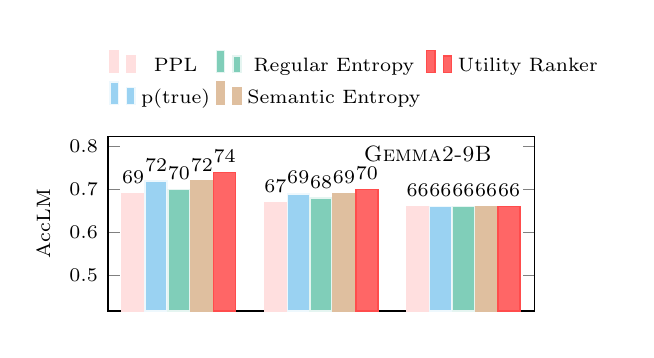
\begin{tikzpicture}
      \begin{axis}[
        ylabel={AccLM},
        major x tick style = transparent,
        ybar = 0.3pt,
        width=7cm,
        bar width=2.8mm,
        height=3.8cm,
        symbolic x coords={accuracy_at_0.8_answer_fraction,accuracy_at_0.9_answer_fraction,accuracy_at_1.0_answer_fraction},
        %xticklabels={80\%, 90\%, 100\%},
        xticklabel=\empty,
        line width=0.5pt,
        xtick = data,
        x tick label style={font=\scriptsize,text width=1cm,align=center, below=-1.5mm},
        y tick label style={font=\scriptsize},
        scaled y ticks = true,
        enlarge x limits=0.25,
        enlarge y limits=0.35,
        ymin=0.5,
ylabel style={font=\scriptsize},
legend columns=2,transpose legend,
 	nodes near coords={
        {\scriptsize \textcolor{black}{\pgfmathprintnumber[precision=1]{\pgfplotspointmeta}}}
       }, %shwowing numbers on top of bars!!!!!
point meta=y *100, % the displayed number,
        %legend cell align = left,
        legend style={
                at={(-0.05,1.0)},
    inner sep=0.8em,
	      anchor=south west ,
              %column sep=1ex,
              draw=none, legend columns=-1,
              font=\scriptsize,
              cells={align=center},
              legend columns = 2,
              transpose legend
        } 
      ]
       \addplot[style={pink!50, fill=pink!50}] plot coordinates {(accuracy_at_0.8_answer_fraction, 0.69) (accuracy_at_0.9_answer_fraction, 0.67) (accuracy_at_1.0_answer_fraction, 0.66)}; %PPL
       \addplot[style={skybleu!10, fill=skybleu!60}] plot coordinates 
       {(accuracy_at_0.8_answer_fraction, 0.72) (accuracy_at_0.9_answer_fraction, 0.69) (accuracy_at_1.0_answer_fraction, 0.66)}; % p(true)
       \addplot[style={bluishGreen!10, fill=bluishGreen!50}] plot coordinates {(accuracy_at_0.8_answer_fraction, 0.7) (accuracy_at_0.9_answer_fraction, 0.68) (accuracy_at_1.0_answer_fraction, 0.66)}; %Regular Entropy
      \addplot[style={brown!50, fill=brown!50}] plot coordinates {(accuracy_at_0.8_answer_fraction, 0.72) (accuracy_at_0.9_answer_fraction, 0.69) (accuracy_at_1.0_answer_fraction, 0.66)}; %Semantic Entropy
      \addplot[style={red!70, fill=red!60}] plot coordinates {(accuracy_at_0.8_answer_fraction, 0.74) (accuracy_at_0.9_answer_fraction, 0.7) (accuracy_at_1.0_answer_fraction, 0.66)}; %Utility Ranker

      \node[above,font=\footnotesize] at ($(current bounding box.north)+(75,0)$) {\textsc{Gemma2-9B}};
            
      \addlegendentry{PPL}
      \addlegendentry{p(true)}
      \addlegendentry{Regular Entropy}
      \addlegendentry{Semantic Entropy}
      \addlegendentry{Utility Ranker}
      
      \end{axis}
    \end{tikzpicture}
  %}
  \\[-1.2ex]
  %\subfloat[\textsc{Llama-3.1-8B}]{
    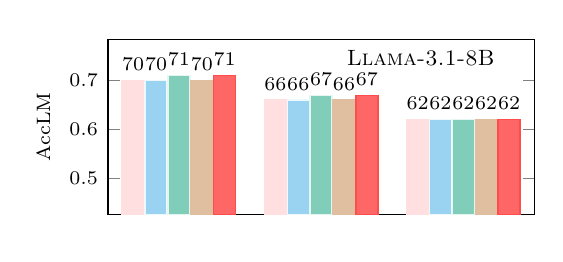
\begin{tikzpicture}
      \begin{axis}[
        ylabel={AccLM},
        major x tick style = transparent,
        ybar = 0.3pt,
        width=7cm,
        bar width=2.8mm,
        height=3.8cm,
        symbolic x coords={accuracy_at_0.8_answer_fraction,accuracy_at_0.9_answer_fraction,accuracy_at_1.0_answer_fraction},
        %xticklabels={80\%, 90\%, 100\%},
        xticklabel=\empty,
        line width=0.5pt,
        xtick = data,
        x tick label style={font=\scriptsize,text width=1cm,align=center, below=-1.5mm},
        y tick label style={font=\scriptsize},
        scaled y ticks = true,
        enlarge x limits=0.25,
        enlarge y limits=0.35,
        ymin=0.5,
ylabel style={font=\scriptsize},
 	nodes near coords={
        {\scriptsize \textcolor{black}{\pgfmathprintnumber[precision=1]{\pgfplotspointmeta}}}
       }, %shwowing numbers on top of bars!!!!!
point meta=y *100, % the displayed number,
        legend cell align = left,
        legend style={
                at={(-0.1,1.0)},
    inner sep=0.8em,
	      anchor=south west ,
              %column sep=1ex,
              draw=none, legend columns=-1,
              font=\scriptsize
        } 
      ]
       \addplot[style={pink!50, fill=pink!50}] plot coordinates {(accuracy_at_0.8_answer_fraction, 0.7) (accuracy_at_0.9_answer_fraction, 0.66) (accuracy_at_1.0_answer_fraction, 0.62)}; %PPL
       \addplot[style={skybleu!10, fill=skybleu!60}] plot coordinates {(accuracy_at_0.8_answer_fraction, 0.7) (accuracy_at_0.9_answer_fraction, 0.66) (accuracy_at_1.0_answer_fraction, 0.62)}; % p(true)
       \addplot[style={bluishGreen!10, fill=bluishGreen!50}] plot coordinates {(accuracy_at_0.8_answer_fraction, 0.71) (accuracy_at_0.9_answer_fraction, 0.67) (accuracy_at_1.0_answer_fraction, 0.62)}; %Regular Entropy
      \addplot[style={brown!50, fill=brown!50}] plot coordinates {(accuracy_at_0.8_answer_fraction, 0.7) (accuracy_at_0.9_answer_fraction, 0.66) (accuracy_at_1.0_answer_fraction, 0.62)}; %Semantic Entropy
      \addplot[style={red!70, fill=red!60}] plot coordinates {(accuracy_at_0.8_answer_fraction, 0.71) (accuracy_at_0.9_answer_fraction, 0.67) (accuracy_at_1.0_answer_fraction, 0.62)};

      \node[above,font=\footnotesize] at ($(current bounding box.north)+(70,0)$) {\textsc{Llama-3.1-8B}};

      \end{axis}
    \end{tikzpicture}
  %}
  \\[-1.2ex]
  %\subfloat[\textsc{Mistral-7B-v0.3}]{
    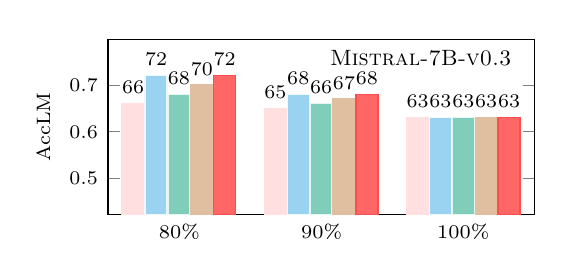
\begin{tikzpicture}
      \begin{axis}[
        ylabel={AccLM},
        major x tick style = transparent,
        ybar = 0.3pt,
        width=7cm,
        bar width=2.8mm,
        height=3.8cm,
        symbolic x coords={accuracy_at_0.8_answer_fraction,accuracy_at_0.9_answer_fraction,accuracy_at_1.0_answer_fraction},
        xticklabels={80\%, 90\%, 100\%},
        line width=0.5pt,
        xtick = data,
        x tick label style={font=\scriptsize,text width=1cm,align=center, below=-1.5mm},
        y tick label style={font=\scriptsize},
        scaled y ticks = true,
        enlarge x limits=0.25,
        enlarge y limits=0.35,
        ymin=0.5,
ylabel style={font=\scriptsize},
 	nodes near coords={
        {\scriptsize \textcolor{black}{\pgfmathprintnumber[precision=1]{\pgfplotspointmeta}}}
       }, %shwowing numbers on top of bars!!!!!
point meta=y *100, % the displayed number,
        legend cell align = left,
        legend style={
                at={(1.15,0.98)},
    inner sep=0.2em,
	      anchor=north ,
              column sep=1ex,
        } 
      ]
       \addplot[style={pink!50, fill=pink!50}] plot coordinates {(accuracy_at_0.8_answer_fraction, 0.66) (accuracy_at_0.9_answer_fraction, 0.65) (accuracy_at_1.0_answer_fraction, 0.63)}; %PPL
       \addplot[style={skybleu!10, fill=skybleu!60}] plot coordinates {(accuracy_at_0.8_answer_fraction, 0.72) (accuracy_at_0.9_answer_fraction, 0.68) (accuracy_at_1.0_answer_fraction, 0.63)}; % p(true)
       \addplot[style={bluishGreen!10, fill=bluishGreen!50}] plot coordinates {(accuracy_at_0.8_answer_fraction, 0.68) (accuracy_at_0.9_answer_fraction, 0.66) (accuracy_at_1.0_answer_fraction, 0.63)}; %Regular Entropy
      \addplot[style={brown!50, fill=brown!50}] plot coordinates {(accuracy_at_0.8_answer_fraction, 0.7) (accuracy_at_0.9_answer_fraction, 0.67) (accuracy_at_1.0_answer_fraction, 0.63)}; %Semantic Entropy
      \addplot[style={red!70, fill=red!60}] plot coordinates {(accuracy_at_0.8_answer_fraction, 0.72) (accuracy_at_0.9_answer_fraction, 0.68) (accuracy_at_1.0_answer_fraction, 0.63)};

      \node[above,font=\footnotesize] at ($(current bounding box.north)+(70,0)$) {\textsc{Mistral-7B-v0.3}};
      
      \end{axis}
    \end{tikzpicture}
  %}

 \vspace*{-1.2cm}
  \captionof{figure}{Average QA model accuracy (AccLM)
    across test sets: models refuse to answer  according
    to different  uncertainty estimation methods. 80/90\%: the 
    model  answers 80/90\% of the questions with low
    uncertainty; 100\%: the model answers all questions.}
\label{fig:main:acc:atX}
\end{figure}


\paragraph{Answering selectively based on Passage Utility improves QA accuracy.}

Answer uncertainty can be used to decide whether to answer or refrain
from doing so. Figure~\ref{fig:main:acc:atX} shows QA model accuracy
across datasets (average AccLM) at different thresholds of answer
rejection. We report accuracy when models choose to answer only 80\%
and 90\% of the cases where they are most certain, and when they
always answer. Across different LLM backbones,
Passage Utility performs on par with or better than more expensive
uncertainty estimation approaches.


\paragraph{Passage Utility performance remains consistent across model sizes.}
Figure~\ref{fig:unc:model:size} (left), shows average AUROC scores on
answer uncertainty estimation for Passage Utility and comparison
approaches with different \textsc{Gemma2} sizes: 2B, 9B, and 27B. Our
Passage Utility approach performs best across model sizes. All
approaches obtain better AUROC scores for the smaller \textsc{Gemma2}
model~(2B) which makes most errors; we observe a noticeable decrease
in performance for most information-theoretic models when using the
biggest \textsc{Gemma} model (27B). We attribute this to the fact that
the 27B model more confidently makes less errors. p(true) on the other
hand benefits from the largest model's context understanding and memorised
knowledge.

 Figure~\ref{fig:unc:model:size} (right) shows average accuracy when
 the target QA models choose to answer~80\% of the cases they are most
 confident about. For comparison, we also show QA accuracy when always
 answering, i.e.,~black bold dots.  When looking at selective
 performance according to Passage Utility, the small
 \textsc{Gemma2-2B} model surpasses the bigger \textsc{Gemma2-27B} one
 when always answering (0.68 vs 0.65), whereas the biggest
 \textsc{Gemma2-27B} model improves by~+9 points (0.74~vs~0.65).


\begin{figure}[t]
    \centering
    \begin{tikzpicture}
\begin{axis}[
height=4.2cm,
width=4cm,
symbolic x coords={\textsc{2B}, \textsc{9B}, \textsc{27B}},
xtick=data,
xticklabel style={anchor=near xticklabel},
%xlabel={QA model size},
extra y tick style={grid=major, tick label style={xshift=-1cm}},
ylabel={Avg AUROC},
ymin=0.5,
y tick label style={font=\scriptsize},
ylabel style={font=\scriptsize},
x tick label style={font=\scriptsize},
xlabel style={font=\scriptsize},
y label style={at={(axis description cs:-0.2,.5)},anchor=south},
legend columns=2,transpose legend,
        %legend cell align = left,
        legend style={
                at={(-0.1,1.0)},
    inner sep=0.8em,
	      anchor=south west ,
              %column sep=1ex,
              draw=none, legend columns=-1,
              font=\scriptsize,
              cells={align=center},
        } 
]
\addplot[pink!50, mark=square*] table[x=date,y=value] {data/auroc_ppl.dat};
\addplot[skybleu!60, mark=triangle*] table[x=date,y=value] {data/auroc_ptrue.dat};
\addplot[bluishGreen!50, mark=*] table[x=date,y=value] {data/auroc_re.dat};
\addplot[brown!50, mark=diamond*] table[x=date,y=value] {data/auroc_se.dat};
\addplot[red!60, mark=10-pointed star] table[x=date,y=value] {data/auroc_utilityranker.dat};
      \addlegendentry{PPL}
      \addlegendentry{p(true)}
      \addlegendentry{Regular Entropy}
      \addlegendentry{Semantic Entropy}
      \addlegendentry{Passage Utility}
\end{axis}
\end{tikzpicture}
\hspace{-4cm}
\begin{tikzpicture}
\begin{axis}[
height=4.2cm,
width=4cm,
symbolic x coords={\textsc{2B}, \textsc{9B}, \textsc{27B}},
xtick=data,
xticklabel style={anchor=near xticklabel},
extra y tick style={grid=major, tick label style={xshift=-1cm}},
ylabel={Avg AccLM on 80\%},
ymin=0.6,
y tick label style={font=\scriptsize},
ylabel style={font=\scriptsize},
x tick label style={font=\scriptsize},
xlabel style={font=\scriptsize},
y label style={at={(axis description cs:-0.25,.5)},anchor=south},
]
\addplot[pink!50, mark=square*] table[x=date,y=value] {data/acc80_ppl.dat};
\addplot[skybleu!60, mark=triangle*] table[x=date,y=value] {data/acc80_ptrue.dat};
\addplot[bluishGreen!50, mark=*] table[x=date,y=value] {data/acc80_re.dat};
\addplot[brown!50, mark=diamond*] table[x=date,y=value] {data/acc80_se.dat};
\addplot[red!60, mark=10-pointed star] table[x=date,y=value] {data/acc80_utilityranker.dat};
\addplot[red!60, mark=10-pointed star] table[x=date,y=value] {data/acc80_utilityranker.dat};
\addplot[only marks] table[x=date,y=value] {data/acc80_acc100.dat};
\end{axis}
\end{tikzpicture}
    \vspace{-1.2cm}
    \caption{(left) Average AUROC for answer uncertainty estimation
      methods with varying \textsc{Gemma2} sizes: 2B, 9B, and
      27B. (right) Average AccLM on the 80\% most confident answers;
      black dots indicate average AccLM when always answering. Results computed on test sets.}
    \label{fig:unc:model:size}
\end{figure}


\paragraph{Passage Utility scores provide good passage re-ranking.}

We hypothesize that by re-ordering the set of retrieved passages
according to their Passage Utility score and filtering the top-$k$
ones, it will be possible to improve the accuracy and efficiency of
the target QA model
\cite{retrieval:quality:eval:siggir,liu-etal-2024-lost}.  To test
this, we measure QA accuracy for \textsc{Gemma2-9B} on sets of input
passages varying in order and size. Specifically, we measure
performance with a set of $|R|=10$ passages in their original ranking
provided by an external retriever and the re-ranking imposed by the
Passage Utility score. We then compute accuracy for the top-$k$
passages with $k$~in the range of \{10, 5, 3, 1\}.
Figure~\ref{fig:unc:rerank} shows average accuracy (AccLM) values
across five datasets (NQ, TQA, WebQ, SQuAD, and PopQA) on different
input sets created based on the original retriever (gray) and the
Passage Utility scores (red).  At $k=10$ both rankings lead to the
same average QA accuracy (67\%). However, when reducing the size of the
context to the top $k=5, 3, 1$ passages re-ranked by the Passage
Utility score, the QA model achieves higher accuracy, indicating that
Passage Utility indeed captures which passages are useful for the
target QA model.

\begin{figure}[t]
    \centering
    \begin{tikzpicture}
\begin{axis}[
height=4.2cm,
width=5.5cm,
symbolic x coords={\textsc{10}, \textsc{5}, \textsc{3}, \textsc{1}},
xtick=data,
xticklabel style={anchor=near xticklabel},
%xlabel={QA model size},
extra y tick style={grid=major, tick label style={xshift=-1cm}},
ylabel={Avg AccLM},
ymin=0.55,
y tick label style={font=\scriptsize},
ylabel style={font=\scriptsize},
x tick label style={font=\scriptsize},
xlabel style={font=\scriptsize},
y label style={at={(axis description cs:-0.2,.5)},anchor=south},
%legend columns=2,transpose legend,
        legend cell align = left,
        legend style={
                at={(-0.2,1.0)},
    inner sep=0.8em,
	      anchor=south west ,
              %column sep=1ex,
              draw=none, legend columns=2,
              font=\scriptsize
        } 
]
\addplot[gray, mark=square*] table[x=date,y=value] {data/acclm_rr_retriever.dat};
\addplot[red!60, mark=10-pointed star] table[x=date,y=value] {data/acclm_rr_pu.dat};
\addlegendentry{Retriever Score}
\addlegendentry{Passage Utility}
\end{axis}
\end{tikzpicture}

    \vspace{-1.2cm}
    \caption{Average retrieval augmented QA accuracy (AccLM) for
      \textsc{Gemma2-9B} across five QA test sets (NQ, TQA, WebQ,
      SQuAD, and PopQA). Points on the x-axis correspond to
      different context sizes~$|R|$, when taking the top-$k$
      passages from  different rankings produced by the retriever and
       Passage Utility estimator; $k$~varies over \{10, 5, 3, 1\}.}
    \label{fig:unc:rerank}
\end{figure}


\paragraph{Training with pairwise judgements on Passage Utility helps improve predictions.}

Table~\ref{tab:main:ragqa-ablation:dev} shows AUROC results on answer
uncertainty prediction with Passage Utility estimators trained with
different variants of the objective in Equation~\eqref{eq:combined}.
The first row shows the full objective (see training details in
Section~\ref{sec:app:implem:det}), the second row shows a variant
where the ranking objective uses only entailment annotations ($e$),
and in the third row the objective is solely based on accuracy
prediction ($\mathcal{L}_{BCE}$). As can be seen, there is a drop in
performance when the pairwise ranking loss is not used (i.e.,~last
line of Table~\ref{tab:main:ragqa-ablation:dev}); this component of
the objective provides a smoother signal on passage utility which is
empirically beneficial. However, when the pairwise ranking loss is
only based on entailment (an external critic), performance drops by
several points which  highlights the importance of training with
utility judgements provided by the target QA model.

\begin{table}[t]
    \small
    \centering
    \begin{tabular}{l|*{3}{c}}
         \hline
          & \textsc{G9B} & \textsc{L8B} & \textsc{M7B}\\ 
        \hline
        $\mathcal{L}_{rank}, (e + a)/2 + \lambda \, \mathcal{L}_{BCE} $ & 0.79 & 0.81 & 0.79 \\
        $\mathcal{L}_{rank}, (e) + \lambda \, \mathcal{L}_{BCE} $  & 0.71 & 0.73 & 0.71 \\
        $\mathcal{L}_{BCE}$  & 0.77 & 0.78 & 0.80\\
        \hline
    \end{tabular}
    %\vspace{-0.2cm}
        \caption{Answer uncertainty estimation with Passage Utility
      predicted by models trained with different variants of the
      training objective in Equation~\ref{eq:combined}. We report AUROC for \textsc{Gemma2-9B (G9B)}, \textsc{Llama3.1-8B (L8B)}, and \textsc{Mistral-7B-v0.3 (M7B)} averaged over development sets.}
      %on the NQ development set.} 
    \label{tab:main:ragqa-ablation:dev}
\end{table}

\section{Conclusions}

In this work we focus on retrieval augmented QA and present an
approach to answer uncertainty prediction that relies on single
passage utilities. We train a small neural model on passage utility
judgements collected from the target QA model. We show that our
uncertainty estimator is competitive or better than existing strong
error prediction methods while being light-weight.  Our experiments
also show that our approach is particularly good in cases of extreme
answer uncertainty such as questions about non-existing entities,
where bigger QA models are prone to confidently formulate an incorrect
answer.  As future work, we would like to explore how to extend our
approach to long-form generation tasks, such as query
focused-summarisation.


\section{Limitations}

Instruction-tuned models are known to refuse to answer questions,
i.e., they produce answers such as ``\textit{This information is not
  available in the text}''. Refusing to answer is an adequate response
when none of the input passages contains appropriate
information. However, in many cases QA models refuse when in fact they
should provide an answer
\citep{adlakha-etal-2024-evaluating,refunq}. Following previous work
\citep{farquhar2024semantic-hallu}, we did not explicitly instruct the
QA models to abstain and consider all cases where the answer does not
match the goldstandard as incorrect. Refusing to answer is in our
setting an indication of uncertainty (i.e.,~the QA model cannot provide a
correct answer) which  we aim to predict.

In this work, we focus on answer uncertainty estimation for short-form
information-seeking QA tasks
\citep{rodriguez-boyd-graber-2021-evaluation} where the answer can be
often found in one Wikipedia passage.  Going forward, it would make
sense to extend our approach to multi-hop and related questions
involving more complex reasoning
\citep{yang-etal-2018-hotpotqa,pmlr-v174-pal22a-medmcqa}.  Although we
expect Passage Utility to be effective in estimating the usefulness of
individual passages, it is also possible that a more complex Passage
Utility aggregation function is required
\citep{dong-etal-2018-confidence}.

% Bibliography entries for the entire Anthology, followed by custom entries
%\bibliography{anthology,custom}
% Custom bibliography entries only
\bibliography{ragu_preprint}


\appendix


\section{Test Time Cost of Uncertainty Estimation Methods}
\label{sec:app:app:cost}

Table~\ref{tab:app:cost} shows the cost of estimating uncertainty for
question~$x$, measured by the number of inference calls
required. Simple information theoretic methods (e.g., PPL) require a
single call to the target QA model with the retrieval augmented QA
prompt (i.e.,~$|R|$ retrieved passages and question $x$). However,
approaches that estimate uncertainty based on diversity (e.g., Regular
Entropy, Semantic Entropy, and p(true)) require generating
$N$~answers, i.e., $N$~inference calls with the retrieval augmented QA
prompt. In addition, Semantic Entropy requires the computation of
answer clusters (i.e., grouping answers with the same meaning), so
additional calls to an entailment model are required to compare the
set of sampled answers. p(true) requires one additional LLM call to
elicit a True/False answer but with a very long prompt including
in-context examples and the assessment question with the $|R|$
retrieved passages, sampled and most likely answers, and question~$x$
(see Table~\ref{tab:ptrue:prompt}). In contrast, our approach requires
$|R|$~utility predictions with a BERT-sized model.

\begin{table}[t]
    \centering
    \small
    \begin{tabular}{l|p{4cm}}
    \hline
    Methods  & \multicolumn{1}{c}{Inference Calls at Test Time} \\ 
    \hline
PPL & $1 \, \text{G}$ \\ 
p(true) & $(N + 1) \, \text{G} + 1 \, \text{E}$ \\
Regular Entropy   & $(N + 1) \, \text{G} $ \\
Semantic Entropy   & $(N + 1) \, \text{G} + {N\choose 2} \, \text{E}$ \\
Passage Utility & $|R| \, \text{Bert-F}$   \\
    \hline
    \end{tabular}
    \caption{Number and type of inference calls required to estimate
      answer uncertainty for question~$x$ and set of retrieved
      passages~$R$. G means inference is performed with a retrieval
      augmented QA model, i.e., a LLM forward pass with the prompt
      including the set of~$|R|$ retrieved passages and question $x$
      to generate a candidate answer~$y$. E is inference with an
      evaluation model, e.g.,~a forward pass to ask an LLM for
      correctness in p(true) or a forward pass with an entailment
      model in Semantic Entropy. Bert-F is an inference call to
      predict passage utility for passages~$p$ in $R$ and
      question~$x$.}
    \label{tab:app:cost}
\end{table}

\section{Experimental Details}

\subsection{Datasets and Splits}
\label{sec:app:datasets}

\begin{table*}[t]
    \centering
    \small
    \begin{tabular}{lrrrp{6cm}p{3.8cm}}
    \hline
    Dataset & \multicolumn{1}{c}{Train} & \multicolumn{1}{c}{Dev} & \multicolumn{1}{c}{Test} & \multicolumn{1}{c}{Example Question} & \multicolumn{1}{c}{Example Answer} \\
    \hline
NQ &  79,168 & 8,757 & 3,610 & Who plays Letty in Bring it on all or nothing? & Francia Raisa \\
TQA &78,785 & 8,837 & 11,313 & Who was the first artistic director of the National Theatre in London? & Lord Laurence Olivier \\
WebQ & 2,474 & 361 & 2,032 & What party was Andrew Jackson? & Democratic-Republican Party \\
SQuAD & 78,713 & 8,886 & 10,570 & What is the Grotto at Notre Dame? & A Marian place of prayer and reflection \\
PopQA & 10,000 & 1,267 & 3,000 & Who was the director of Champion? & Rabi Kinagi \\
RefuNQ & --- & --- & 2,173 & Who does the voice over in the Requirtion? & --- \\
\hline
    \end{tabular}
    \caption{Dataset statistics, number of instances per
      Train/Development(Dev)/Test sets, and example question-answer
      pairs (all taken from the Dev set except for RefuNQ).} 
    \label{tab:datasets:stat}
\end{table*}

In our experiments, we use six QA tasks which we describe below. Table~\ref{tab:datasets:stat} shows dataset statistics and example question-answers pairs. 

\paragraph{Natural Questions} (NQ;
\citealt{kwiatkowski-etal-2019-natural}) is a QA dataset compiled from
real user questions submitted to the Google search engine. As
part of the dataset curation process, annotators judge the quality of
questions and associate them with a short answer that can be extracted
from a related Wikipedia page.  
%These questions are impresice and ambiguous, there is answer variability, experiments in the original paper on this.

\paragraph{TriviaQA} (TQA; \citealt{joshi-etal-2017-triviaqa})  is a  question answering dataset designed for training and evaluating machine learning models on open-domain question answering tasks. The dataset was created by gathering questions from trivia websites, along with their corresponding answers, to provide a broad range of factual questions.
% questions are supposed to be more complex, requiering complex reasoning over several sentences from the evidence and lexical variation of the answer w.r.t the evidence paragraph.

\paragraph{WebQuestions} (WebQ; \citealt{berant-etal-2013-semantic})
was mined off questions generated with the Google Suggest API. The
answers to the questions are defined as Freebase entities (i.e., their
string label) and were elicited by Amazon Mechanical Turk (AMT)
annotators.
%in some cases answers are roughly accurate as AMT workers are obliged to select entities only from Freebase. Also list of entities might be incomplete.

\paragraph{SQuAD} \citep{rajpurkar-etal-2016-squad} contains questions
formulated by AMT annotators based on a given Wikipedia paragraph,
with the answer being a short span in that paragraph. Annotators were
encouraged to use paraphrasing when writing the question. The answer
types not only cover named entities but also other categories such as
noun- and verb-phrases.
% variety of answer types (noun- and verb- phrases). questions and paragraphs' lexical & syntactic divergence, multi-sentence reasoning, ambiguos questions (small percentage).

\paragraph{PopQA} \cite{mallen-etal-2023-popQA} is an open-domain QA
dataset, focusing on popular culture topics, such as movies, TV shows,
music, and sports. It  contains question-answer pairs derived from (subject,
relation, object) triples in Wikidata . Triples were translated into
natural language and the object entity was taken to be the gold
answer. The collection process focused on gathering questions about
subject entities of varying popularity. 

\paragraph{RefuNQ} \cite{refunq} is derived from NQ and consists of answerable and unanswerable questions. Unanswerable questions are created by replacing entities in the original NQ question by non-existing concepts.


We follow previous work \citep{lee-etal-2019-latent} and use only the
question and gold answers, i.e., the open versions of NQ, TQA, and
SQuAD. We use the unfiltered TQA dataset. We follow the train/dev/test
splits as used in previous work \cite{lee-etal-2019-latent} and randomly split PopQA. RefuNQ only provides a test set so our experiments on this dataset 
are zero-shot from a Passage Utility predictor trained on SQuAD.
We follow \citet{farquhar2024semantic-hallu} and use 400 test examples 
randomly sampled from the original larger test datasets for evaluation of uncertainty quantification.

\subsection{Implementation Details}
\label{sec:app:implem:det}

\paragraph{QA Models}

For all question answering tasks, we use the off-the-shelf
Contriever-MSMARCO \citep{izacard2022unsupervised} tool to retrieve sets of
passages~$R$ for question~$x$ from Wikipedia and the official
Wikipedia embeddings based (2018 snapshot) as our document
knowledge-base. For PopQA, we follow the work by
\citet{mallen-etal-2023-popQA} who also use the full 2018 English
Wikipedia dump.

The QA prompt used for all models (embedded in the corresponding chat templates) is shown in Table~\ref{tab:ragu_prompts}.
For inference, we set the maximum number of generated tokens to 50 for both the greedy (most likely answer) as well as temperature scaled (sampled candidates) decoding. We use vLLM for inference \citep{vllm}. For all models, inference was run on a single A100-80GB GPU.

\paragraph{Passage Utility Predictor}

We train a different predictor for each target QA model and QA
task. Given the large number of predictors required in  our
experiments, we initially tested the hyper-parameters used in
\citet{fang-etal-2024-efficiently} on the NQ dataset and choose a set
thereof for all predictor instances. We train each predictor for 3
epochs, with a batch size of 32 examples, learning rate equal to
2$^{e-5}$, and weight decay 0.001.
%(e.g., weight decay 0.01 yield
%models with more variance).
For each predictor we performed search on values for $\lambda$, i.e., the
contribution of the $\mathcal{L}_{BCE}$ loss
(Equation~\ref{eq:combined}), and different criteria for model
selection, i.e., the best at pairwise ranking or at both pairwise
ranking and accuracy prediction
(combined).

Table~\ref{tab:model:select} shows the configuration for each
predictor. Table cells show selection criteria (R for ranking and C
for combined) and the value for~$\lambda$. A trend that seems to
emerge for \textsc{Llama-3.1-8B} and \textsc{Mistral-7B-v0.3} is that
best predictors tend to rely more on the target QA model accuracy,
potentially indicating that their answers in some cases depend less on
context. However, for the smaller model \textsc{Gemma2-2B} all
predictors achieve a good ranking, which supports the hypothesis that
small models rely more on the provided content to formulate their
answers. At inference time we predict a single Passage Utility score 
given by the selected best checkpoint.
For all predictor instances (except for all WebQ and PopQA predictors and
the predictor for \textsc{Llama-3.1-8B} and NQ),  we use half of the
available training data to speed up experiments. Training and inference was run on a single A100-40GB GPU, training takes less than 12 hours depending on the dataset.


\begin{table}[t]
    \centering
    \small
    \begin{tabular}{@{}l@{~}c@{~~}c@{~}c@{~}c@{~}c@{}}
         \hline
       \multicolumn{1}{c}{Models} & NQ & TQA & WebQ & SQuAD & PopQA \\ 
        \hline \\[-1.2ex]

        \textsc{Gemma2.9B} & R, 0.25 & R, 0.25 & C, 1 & C, 1 & R, 0.25 \\      
        
        \textsc{Llama-3.1-8B} & C, 0.25 & C, 1 & R, 0.25 & C, 1 & C, 1 \\
        
        {\textsc{Mistral-7B-v0.3}} & R, 0.25 & C, 1 & R, 0.25 & C, 1 & C, 1 \\[0.4ex]

        \textsc{Gemma2.2B} & R, 0.25 & R, 0.25 & R, 0.25 & R, 0.25 & R, 0.25 \\    

        \textsc{Gemma2.27B} & R, 0.25 & C, 1 & C, 1 & R, 0.25 & R, 0.25 \\   
\hline
    \end{tabular}
    \caption{This table shows the $\lambda$ value and selection criteria (R for pairwise ranking or C for combined pairwise ranking and accuracy prediction) for each Passage Utility predictor in our experiments.}
    \label{tab:model:select}
\end{table}

\paragraph{Comparison Approaches}

In the additional results section of the appendix
(Section~\ref{sec:app:additionalres:unc}), we report the following
additional answer uncertainty estimation methods.  Maximum Sequence
Probability (MSP) is based on the probability of the most likely
answer and is computed as
\begin{equation}
\text{MSP}(x, R, \mathcal{M}) = 1 - P(y | x, R; \mathcal{M}).    
\end{equation}
Note that, in contrast to $PPL(x, R, \mathcal{M})$ reported in the
main section of the paper, this metric is biased by answer length,
i.e., identifying an answer to have low probability (low confidence)
because of its length. Despite the fact that QA models are instructed
to produce short answers, they do not always follow instructions. For
this reason, we consider perplexity a more accurate metric. Indeed,
the length of the answer could be a feature indicating that the model
is uncertain about the answer.

We estimate answer uncertainty from the Average Answer Length
(Avg.Ans.Len) as the average number of words in the sampled
answers. We also report Cluster Assignment (CA) which is a variant of
SE without answer probabilities where the probability of each
generated meaning (i.e., a cluster) is approximated from the number of
answers in the cluster. We found that in general CA estimations are
very close to Semantic Entropy ones.


Another uncertainty estimation approach is the negative mean
Point-wise Mutual Information (PMI;
\citealt{takayama-arase-2019-relevant}) over tokens; i.e.,~it compares
the probability of answer sequence $y$ given a prompt with question
$x$ and passages $R$ w.r.t the probability given by $\mathcal{M}$ to
$y$ without any context. Intuitively, the higher the point-wise mutual
information, the more certain the QA model is on generating $y$ (i.e.,
the answer is related to or depends on $x$ and $R$). PMI is computed
as
\begin{equation}
\begin{aligned}
\text{PMI}(x, R, \mathcal{M}) =   \\ - \, \frac{1}{|y|} \sum_{t=1}^{|y|} \text{log} \dfrac{p(y_t|y_{1..t-1}, x, R; \mathcal{M})}{p(y_t|y_{1..t-1};\mathcal{M})} .   
\end{aligned}
\end{equation}
 

We use the implementation provided by \citet{farquhar2024semantic-hallu} to compute Regular Entropy, Semantic Entropy, Cluster Assignment, and p(true). 


\paragraph{Metrics}
We use the implementation provided by \citet{farquhar2024semantic-hallu} for the AUROC, Accuracy at X\% of rejection, and AURAC metrics.

We use Qwen2-72B-Instruct \citep{qwen2} to obtain accuracy judgments
(i.e., $A$ judge, Section~\ref{sec:experimental});
specifically, we use the Activation-aware Weight Quantization
\citep{awq} version Qwen2-72B-Instruct-AWQ.  We prompt the accuracy
evaluator with the prompt proposed by \citet{sun-etal-2024-head}, as
we found it to perform well. The accuracy evaluation (AccLM) prompt is
shown in Table~\ref{tab:acclm}.  In a sample of 840 generated answers
human and LLM-based judgment of correctness agreed 98\% of the time
\citep{sun-etal-2024-head}.  As a reference point, to relate to
accuracy as computed in previous work, we report retrieval augmented
QA accuracy (\textbf{Acc}) defined as whether the gold answer is
contained in the generated answer \citep{mallen-etal-2023-popQA,
  asai2024selfrag}.

\begin{table}[t]
    \centering
    \footnotesize
\begin{promptbox}[colback=white, left=1mm, right=1mm]{Retrieval augmented QA prompt}
Knowledge: \\ \
[1] \textcolor{blue}{passage} \\ \
[2] \textcolor{blue}{passage} \\ \
... \\ \
[$|R|$] \textcolor{blue}{passage} \\ \
 \\ \
Answer the following question with a very short phrase. \\ \
 \\ \
Question: \textcolor{blue}{question} \\
\end{promptbox}
    \caption{Prompt designed as user turn for QA models.}
    \label{tab:ragu_prompts}
\end{table}


\begin{table}[t]
    \centering
    \footnotesize
\begin{promptbox}[colback=white, left=1mm, right=1mm]{p(true) prompt}
Question: \textcolor{blue}{question} \\
Brainstormed Answers: \textcolor{blue}{most likely answer} \\
\textcolor{blue}{sampled answer 1} \\
... \\
\textcolor{blue}{sampled answer N} \\
Possible answer: \textcolor{blue}{most likely answer} \\
Is the possible answer: \\
A) True \\
B) False \\
The possible answer is: \textcolor{blue}{correct choice} \\
\\ \
... \\ \
\\ \
Knowledge: \\ \
[1] \textcolor{blue}{passage} \\ \
[2] \textcolor{blue}{passage} \\ \
... \\ \
[$|R|$] \textcolor{blue}{passage} \\ \
\\ 
Question: \textcolor{blue}{question} \\
Brainstormed Answers: \textcolor{blue}{most likely answer} \\
\textcolor{blue}{sampled answer 1} \\
... \\
\textcolor{blue}{sampled answer $N$} \\
Possible answer: \textcolor{blue}{most likely answer} \\
Is the possible answer: \\
A) True \\
B) False \\
The possible answer is: \\
\end{promptbox}
    \caption{Prompt used for the p(true) comparison approach. The
      items in blue are filled in with in-context examples from the
      training set and the current example being evaluated. $N$ represents
      the number of sampled answers. The 'sequence of in-context
      examples' prefix is a sequence of examples taken from the
      training split with the same question format but with the answer
      to \emph{The possible answer is:} resolved.}
    \label{tab:ptrue:prompt}
\end{table}


\begin{table}[ht]
    \centering
    \footnotesize
\begin{promptbox}[colback=white, left=1mm, right=1mm]{Accuracy evaluation (AccLM) prompt}
You need to check whether the prediction of a question-answering system to a question is correct. You should make the judgment based on a list of ground truth answers provided to you. Your response should be "correct" if the prediction is correct or "incorrect" if the prediction is wrong.\\
\ \\
Question: Who authored The Taming of the Shrew (published in 2002)?\\
Ground truth: ["William Shakespeare", "Roma Gill"]\\
Prediction: W Shakespeare\\
Correctness: correct\\
\ \\
Question: Who authored The Taming of the Shrew (published in 2002)?\\
Ground truth: ["William Shakespeare", "Roma Gill"]\\
Prediction: Roma Gill and W Shakespeare\\
Correctness: correct\\
\ \\
Question: Who authored The Taming of the Shrew (published in 2002)?\\
Ground truth: ["William Shakespeare", "Roma Gill"]"\\
Prediction: Roma Shakespeare\\
Correctness: incorrect\\
\ \\
Question: What country is Maharashtra Metro Rail Corporation Limited located in?\\
Ground truth: ["India"]\\
Prediction: Maharashtra\\
Correctness: incorrect\\
\ \\
Question: What's the job of Song Kang-ho in Parasite (2019)?\\
Ground truth: ["actor"]\\
Prediction: He plays the role of Kim Ki-taek, the patriarch of the Kim family.\\
Correctness: correct\\
\ \\
Question: Which era did Michael Oakeshott belong to?\\
Ground truth: ["20th-century philosophy"]\\
Prediction: 20th century."\\
Correctness: correct\\
\ \\
Question: Edward Tise (known for Full Metal Jacket (1987)) is in what department?\\
Ground truth: ["sound department"]\\
Prediction: 2nd Infantry Division, United States Army\\
Correctness: incorrect\\
\ \\
Question: What wine region is Finger Lakes AVA a part of?\\
Ground truth: ["New York wine"]\\
Prediction: Finger Lakes AVA\\
Correctness: incorrect\\
\ \\
Question: \textcolor{blue}{question}\\
Ground truth: \textcolor{blue}{gold answer}\\
Prediction: \textcolor{blue}{generated answer}\\
Correctness:\\
\end{promptbox}
    \caption{Prompt used for LLM-based accuracy evaluation (AccLM).}
    \label{tab:acclm}
\end{table}



\subsection{Prompts}
\label{sec:app:prompts}


The prompt we use for our QA models is shown in Table~\ref{tab:ragu_prompts}. 
Table~\ref{tab:ptrue:prompt} illustrates the prompt used for our the p(true) baseline.
Table~\ref{tab:acclm} shows the prompt used for the LLM-based accuracy (AccLM) metric.

\section{Additional Results}
\label{sec:app:additionalres}

\subsection{Generalisation of Uncertainty Estimation}
\label{sec:app:generalisation}

In this series of experiments, we assess the generalisation ability of
our Passage Utility estimator. To this end, following previous work on
question answering and out-of-distribution (o.o.d) scenarios
\citep{kamath-etal-2020-selective,zhang-etal-2021-knowing}; we train a
Passage Utility predictor on the SQuAD dataset and then use it to
predict zero-shot (i.e., without further fine-tuning) passage
utilities on all other datasets' test cases. As p(true) relies on 20 in context
training examples, we also evaluate its ability to generalise to out
of distribution test cases.

Table~\ref{tab:main:unc:ood:test} shows AUROC for answer uncertainty
prediction on o.o.d scenarios. We also report PPL as a baseline and
the AUROC values for the in distribution scenario as upper-bound.  
Although Passage Utility performance decreases in o.o.d
settings, it remains competitive in three out of five datasets. On NQ and WebQ the performance is slightly above the PPL baseline. 
Note that we focus on zero-shot accuracy to
assess bare transfer performance; however, it would make sense to
adapt the model with few examples from the o.o.d data
\citep{kamath-etal-2020-selective,zhang-etal-2021-knowing}.
Interestingly, p(true)'s performance also drops in all o.o.d test sets showing that relying on a fixed number of training examples is neither robust nor has a principled and scalable adaptation method (e.g., fine-tuning).

\begin{table*}[t]
    \small
    \centering
    \begin{tabular}{l*{5}{c}}
         \hline
        & NQ & TQA & WebQ & PopQA & RefuNQ  \\ 
        \hline
PPL & 0.64 & 0.68 & 0.52 & 0.59 & 0.51 \\
p(true) (i.i.d) & 0.73 & 0.75 & 0.67 & 0.81 & --- \\
Passage Utility (i.i.d) & 0.72 & 0.82 & 0.70 & 0.84 & --- \\
p(true) (o.o.d) & 0.67 & 0.63 & 0.63 & 0.72 & 0.62 \\     
Passage Utility (o.o.d) & 0.66 & 0.82 & 0.57 & 0.73 & 0.81 \\
        \hline
    \end{tabular}
    \caption{Out-of-domain performance of Passage Utility predictor
      (with \textsc{Gemma2-9B}). Uncertainty predictors are trained on
      SQuAD and evaluated zero-shot on NQ, TQA, WebQ,
      PopQA, and RefuNQ test sets.}
    \label{tab:main:unc:ood:test}
\end{table*}



\subsection{Reference Retrieval Augmented QA Accuracy}
\label{sec:app:additionalres:refacc}

Table~\ref{tab:main:ragqa-perfor} shows retrieval augmented QA performance (Acc and AccLM) for the five QA models on the development and test sets of the six QA tasks. 


\subsection{Detailed Uncertainty Estimation Results}
\label{sec:app:additionalres:unc}


Table~\ref{tab:main:unc:gemma29bit:dev} shows performance of uncertainty quantification approaches on the development sets. We report AUROC and AURAC.


\begin{table*}[t]
    \small
    \centering
    \begin{tabular}{l*{12}{c}}
         \hline
        & \multicolumn{2}{c}{NQ} & \multicolumn{2}{c}{TQA} & \multicolumn{2}{c}{WebQ}  &  \multicolumn{2}{c}{SQuAD} &  \multicolumn{2}{c}{PopQA} &  \multicolumn{2}{c}{RefuNQ} \\ 
        & {\scriptsize Acc} & {\scriptsize AccLM} & {\scriptsize Acc} & {\scriptsize AccLM} & {\scriptsize Acc} & {\scriptsize AccLM} & {\scriptsize Acc} & {\scriptsize AccLM} & {\scriptsize Acc} & {\scriptsize AccLM} & {\scriptsize Acc} & {\scriptsize AccLM}\\ 
        \hline \\[-1.2ex]
        & \multicolumn{12}{c}{Development} \\[0.4ex]
        \hline
        \textsc{Gemma2.9B} & 0.48 & 0.66 & 0.74 & 0.80 & 0.46 & 0.66 & 0.38 & 0.60 & 0.51 & 0.52 & --- & --- \\      
        
        \textsc{Llama-3.1-8B} & 0.48 & 0.62 & 0.71 & 0.77 & 0.53 & 0.64 & 0.39 & 0.57 & 0.51 & 0.49 & --- & --- \\
        
        \textsc{Mistral-7B-v0.3} & 0.48 & 0.62 & 0.72 & 0.76 & 0.52 & 0.69 & 0.37 & 0.58 & 0.53 & 0.51 & --- & --- \\[0.4ex]

        \textsc{Gemma2.2B} & 0.43 & 0.59 & 0.67 & 0.73 & 0.47 & 0.65 & 0.34 & 0.55 & 0.48 & 0.49 & --- & --- \\    

        \textsc{Gemma2.27B} & 0.48 & 0.66 & 0.75 & 0.81 & 0.49 & 0.67 & 0.38 & 0.60 & 0.52 & 0.52 & --- & --- \\    

        \hline \\[-1.2ex]
        & \multicolumn{12}{c}{Test} \\[0.4ex]
        \hline
        \textsc{Gemma2.9B} & 0.49 & 0.65 & 0.74 & 0.80 & 0.40 & 0.66 & 0.43 & 0.60 & 0.50 & 0.52 & 0.26 & 0.40 \\

        \textsc{Llama-3.1-8B} & 0.49 & 0.61 & 0.71 & 0.77 & 0.44 & 0.63 & 0.43 & 0.58 & 0.50 & 0.49 & 0.27 & 0.36 \\

        \textsc{Mistral-7B-v0.3} & 0.49 & 0.62 & 0.72 & 0.77 & 0.47 & 0.66 & 0.41 & 0.58 & 0.51 & 0.50 & 0.26 & 0.35 \\

        \textsc{Gemma2.2B} & 0.44 & 0.57 & 0.67 & 0.72 & 0.39 & 0.61 & 0.39 & 0.56 & 0.48 & 0.49 & 0.24 & 0.33 \\

        \textsc{Gemma2.27B} & 0.48 & 0.65 & 0.76 & 0.81 & 0.41 & 0.66 & 0.42 & 0.61 & 0.51 & 0.53 & 0.26 & 0.39 \\
        
        \hline
\end{tabular}
    \caption{Performance of target QA models (with $|R|=5$) on the development and test sets. We report token- and model-based accuracy (Acc and AccLM). AccLM is computed by Qwen2-72B-Instruct.}
    \label{tab:main:ragqa-perfor}
\end{table*}


\begin{table*}[ht]
    \footnotesize
    \centering
  \begin{tabular}{@{}l@{\hspace{7pt}}c@{\hspace{6pt}}c@{\hspace{4pt}}c@{\hspace{4pt}}c@{\hspace{4pt}}c@{\hspace{4pt}}|c@{\hspace{6pt}}c@{\hspace{4pt}}c@{\hspace{4pt}}c@{\hspace{4pt}}c@{\hspace{4pt}}c@{}} \\
  \hline \ \\[-1ex]
         & NQ & TQA & WebQ  &  SQuAD & PopQA 
         & NQ & TQA & WebQ  &  SQuAD & PopQA \\
  & \multicolumn{5}{c|}{AUROC} & \multicolumn{5}{c}{AURAC} \\
  \hline \ \\[-1.9ex]
        \multicolumn{1}{l}{} &\multicolumn{10}{c}{\textsc{Gemma2-9B}} \\
  \hline
PPL & 0.61 & 0.52 & 0.58 & 0.66 & 0.56 & 0.67 & 0.78 & 0.67 & 0.65 & 0.52 \\
MSP & 0.64 & 0.60 & 0.64 & 0.71 & 0.61 & 0.69 & 0.80 & 0.69 & 0.67 & 0.56 \\
PMI & 0.53 & 0.46 & 0.52 & 0.50 & 0.48 & 0.64 & 0.75 & 0.64 & 0.57 & 0.50 \\
p(true) & 0.70 & 0.71 & 0.66 & 0.73 & 0.83 & 0.72 & 0.84 & 0.70 & 0.69 & 0.71 \\
Regular Entropy & 0.64 & 0.54 & 0.60 & 0.70 & 0.58 & 0.69 & 0.78 & 0.68 & 0.67 & 0.54 \\
Cluster Assignment & 0.68 & 0.65 & 0.65 & 0.70 & 0.68 & 0.71 & 0.82 & 0.70 & 0.67 & 0.60 \\
Semantic Entropy & 0.67 & 0.69 & 0.64 & 0.72 & 0.69 & 0.71 & 0.84 & 0.69 & 0.68 & 0.61 \\
Avg.Ans.Len & 0.61 & 0.64 & 0.65 & 0.63 & 0.68 & 0.68 & 0.83 & 0.71 & 0.65 & 0.61 \\
Passage Utility & \textbf{0.71} & \textbf{0.83} & \textbf{0.71} & \textbf{0.83} & \textbf{0.86} & \textbf{0.74} & \textbf{0.88} & \textbf{0.75} & \textbf{0.76} & \textbf{0.72} \\


\hline \ \\[-1.9ex]
\multicolumn{1}{l}{} &\multicolumn{10}{c}{\textsc{Llama-3.1-8B}} \\
\hline
PPL & 0.75 & 0.78 & 0.68 & 0.75 & 0.81 & 0.76 & 0.85 & 0.71 & 0.71 & 0.68 \\
MSP & 0.77 & 0.80 & 0.71 & 0.76 & \textbf{0.85} & 0.76 & 0.85 & 0.72 & 0.72 & 0.70 \\
PMI & 0.55 & 0.52 & 0.48 & 0.54 & 0.58 & 0.64 & 0.73 & 0.60 & 0.61 & 0.53 \\
p(true) & \textbf{0.80} & \textbf{0.86} & 0.73 & \textbf{0.82} & \textbf{0.85} & \textbf{0.78} & \textbf{0.87} & 0.75 & \textbf{0.75} & \textbf{0.71} \\
Regular Entropy & 0.77 & 0.80 & 0.69 & 0.76 & 0.83 & 0.76 & 0.85 & 0.71 & 0.72 & 0.69 \\
Cluster Assignment & 0.75 & 0.83 & 0.69 & 0.75 & 0.82 & 0.75 & 0.85 & 0.71 & 0.71 & 0.67 \\
Semantic Entropy & 0.74 & 0.83 & 0.69 & 0.74 & 0.81 & 0.75 & 0.86 & 0.71 & 0.71 & 0.68 \\
Avg.Ans.Len & 0.73 & 0.73 & 0.69 & 0.69 & 0.84 & 0.73 & 0.82 & 0.71 & 0.67 & 0.69 \\
Passage Utility & 0.79 & 0.84 & \textbf{0.76} & \textbf{0.82} & \textbf{0.85} & 0.77 & \textbf{0.87} & \textbf{0.76} & 0.74 & 0.70 \\
\hline 
\multicolumn{1}{l}{} &\multicolumn{10}{c}{\textsc{Mistral-7B-v0.3}} \\
\hline
PPL & 0.66 & 0.70 & 0.60 & 0.63 & 0.66 & 0.69 & 0.84 & 0.72 & 0.63 & 0.63 \\
MSP & 0.70 & 0.75 & 0.65 & 0.71 & 0.77 & 0.70 & 0.85 & 0.73 & 0.68 & 0.67 \\
PMI & 0.38 & 0.33 & 0.42 & 0.42 & 0.30 & 0.53 & 0.68 & 0.62 & 0.52 & 0.39 \\
p(true) & 0.72 & \textbf{0.82} & 0.71 & 0.75 & 0.74 & 0.71 & \textbf{0.87} & 0.76 & 0.71 & 0.64 \\
Regular Entropy & 0.67 & 0.71 & 0.63 & 0.66 & 0.68 & 0.69 & 0.85 & 0.73 & 0.66 & 0.63 \\
Cluster Assignment & 0.72 & 0.81 & 0.68 & 0.73 & 0.76 & 0.71 & \textbf{0.87} & 0.75 & 0.68 & 0.66 \\
Semantic Entropy & 0.72 & 0.80 & 0.68 & 0.73 & 0.76 & 0.71 & \textbf{0.87} & 0.76 & 0.69 & 0.66 \\
Avg.Ans.Len & 0.66 & 0.75 & 0.65 & 0.68 & 0.81 & 0.69 & 0.85 & 0.73 & 0.67 & 0.70 \\
Passage Utility & \textbf{0.77} & 0.81 & \textbf{0.74} & \textbf{0.83} & \textbf{0.84} & \textbf{0.74} & \textbf{0.87} & \textbf{0.79} & \textbf{0.74} & \textbf{0.71} \\



\hline
\end{tabular}
    \caption{Answer uncertainty estimation for QA models \textsc{Gemma2-9B}, \textsc{Llama-3.1-8B}, and \textsc{Mistral-7B-v0.3} on NQ, TQA, WebQ, SQuAD, and PopQA development sets. We report AUROC and AURAC. 
    }
    \label{tab:main:unc:gemma29bit:dev}
\end{table*}

\section{Examples of False Positives and Negatives}
\label{sec:app:unc:examples}

Tables~\ref{tab:ex:TN:squad:llama318bit}--\ref{tab:ex:FN:tqa:gemma29bit}
illustrate the working of Passage Utility for answer uncertainty
estimation.  As we report AUROC scores, we do not set any
correct/incorrect decision threshold; for the purpose of this
discussion, we assume a decision point at 0.5 and analyse clear success
and failure cases. For each example, we show the question, gold, and
generated answers in the top block. Then, we show three retrieved
passages with their estimated Passage Utility and a final block with
the ten sampled answers, their grouping into clusters, and the Cluster
Assignment entropy.

Table~\ref{tab:ex:TN:squad:llama318bit} shows an example for a SQuAD
question and the \textsc{Llama-3.1-8B} QA model. In this case, the QA
model correctly answers and the Passage Utility estimate is high
(i.e., indicating correct
answer). Table~\ref{tab:ex:TP:squad:llama318bit} illustrates a case
where \textsc{Llama-3.1-8B}'s answer is incorrect and all Passage
Utilities are very low (i.e., indicating incorrect answer).  The
example from NQ in Table~\ref{tab:ex:FP:nq:gemma29bit} shows a case
where all Passage Utilities are low but the QA model
(\textsc{Gemma2-9B}) answers correctly. The first passage is not
useful, the second does not explicitly mention the answer but still
primes the QA model to  answer correctly, while the third passage 
mentions the answer.

In Table~\ref{tab:ex:FN:tqa:gemma29bit},
Passage Utility scores are high estimating a correct answer for the
TQA test question; however, \textsc{Gemma2-9B} answers with the
incorrect magazine name. Note that none of the passages corresponds to
the National Geographic magazine but have high token overlap with the
question (in particular the first and second passages). 


% Example TN by Passage Utility 
\begin{table*}
\tcbset{colback=white,colframe=green!45!black}
\begin{tcolorbox}[arc=4mm,outer arc=1mm, top=1mm, bottom=1mm]
\begin{flushleft}
\footnotesize{Question: Due to increased unemployment, who mainly opposed the Shah's regime?\\
Generated Answer: Millions of youth and poor migrants.\\
Gold Answer: Millions of youth who had migrated to the cities.}\end{flushleft}
\end{tcolorbox}
\vspace{-.2cm}
\begin{tcolorbox}[colback=white,colframe=green!45!black,enhanced,title=\texttt{\scriptsize Youth who migrated to cities for construction jobs.}, boxed title style={colback=black}, colbacktitle=white, coltitle=black, left=1mm, top=1mm, right=1mm]
\scriptsize{\texttt{Iran. unemployment, especially among millions of youth who had migrated to the cities of Iran  looking for construction jobs during the boom years of the early 1970s. By the late 1970s, many of these people opposed the Shah's regime and began to organize and join the protests against it. The 1979 Revolution, later known as the ``Islamic Revolution'', began in January 1978 with the first major demonstrations against the Shah. [cont.]
\hfill \textcolor{blue}{\texttt 3.93}}}
\vspace*{-.1cm}
\end{tcolorbox}
\vspace{-.2cm}
\begin{tcolorbox}[colback=white,colframe=red,enhanced,title=\texttt{\scriptsize{Unemployed and the poor.}},
boxed title style={colback=white}, colbacktitle=white, coltitle=black, left=1mm, top=1mm, right=1mm]
\scriptsize{\texttt{Ruhollah Khomeini. unemployment, ideological disagreement over the economy, and ``international pressure and isolation'' such as US sanctions following the hostage crisis. Due to the Iran–Iraq War, poverty is said to have risen by nearly 45\% during the first 6 years of Khomeini's rule. Emigration from Iran also developed, reportedly for the first time in the country's history. Since the revolution and war with Iraq, an estimated ``two to four million entrepreneurs, professionals, technicians, and skilled craftspeople (and their capital)'' have emigrated to other countries. [cont.]\hfill \textcolor{blue}{\texttt -1.37}}}
\vspace*{-.1cm}
\end{tcolorbox}
\vspace{-.2cm}
\begin{tcolorbox}[colback=white,colframe=red,enhanced,title=\texttt{\scriptsize{The National Front.}},
boxed title style={colback=red}, colbacktitle=white, coltitle=black, left=1mm, top=1mm, right=1mm]
  \scriptsize{\texttt{Mohammad Reza Pahlavi. professors issued a public statement criticising the 1953 coup, all were dismissed from their jobs, but in the first of his many acts of ``magnanimity'' towards the National Front, Mohammad Reza intervened to have them reinstated. Mohammad Reza tried very hard to co-opt the supporters of the National Front by adopting some of their rhetoric and addressing their concerns, for example declaring in several speeches his concerns about the Third World economic conditions and poverty which prevailed in Iran, a matter that had not much interested him before. [cont.] \hfill \textcolor{blue}{\texttt -3.48}}}
\end{tcolorbox}
\vspace{-.2cm}
\begin{tcolorbox}[colback=white,colframe=red,enhanced, left=1mm, top=1mm, right=1mm]
\scriptsize{\texttt{['Migrants to the cities.'], ['Millions of youth who had migrated to cities.', 'Millions of youth who migrated to cities.'], ['Cultural and religious conservatives, and the urban poor who had migrated to cities for jobs.'],  ['Youth who had migrated to the cities.'], ['Millions of young migrants who had moved to cities in the early 1970s.'], ['Millions of youth and poor migrants to cities.'], ['Cultural and religious conservatives, mostly urban migrants.', 'Cultural and religious conservatives, particularly the migrants to cities.', 'Cultural and religious conservatives, especially those recently migrated to the cities.']\hfill \textcolor{blue}{\texttt 1.83}}}
%[0, 1, 2, 1, 3, 4, 5, 6, 3, 3]
\end{tcolorbox}
    \caption{True negative example (from SQuAD development set): Passage Utility predicts the right answer as well as the  QA model (\textsc{Llama-3.1-8B}).}
    \label{tab:ex:TN:squad:llama318bit}
\end{table*}

% Example TP by Passage Utility 
\begin{table*}
\tcbset{colback=white,colframe=red}
\begin{tcolorbox}[arc=4mm,outer arc=1mm, top=1mm, bottom=1mm]
\begin{flushleft}
\footnotesize{Question: Which company was targeted by the NAACP for not having fair practices?\\
Generated Answer: Target Corporation.\\
Gold Answer: Lockheed Aircraft Corporation.}\end{flushleft}
\end{tcolorbox}
\vspace{-.2cm}
\begin{tcolorbox}[colback=white,colframe=red,enhanced,title=\texttt{\scriptsize Target Corporation.}, boxed title style={colback=black}, colbacktitle=white, coltitle=black, left=1mm, top=1mm, right=1mm]
\scriptsize{\texttt{Target Corporation. of Colored People has repeatedly given Target failing grades on its annual Economic Reciprocity Initiative report card, a measure of the company's ``commitment to the African-American citizenry''. In 2003 and 2005, the NAACP has rated Target an ``F'' on this report; in 2004, Target was rated a ``D-''. In 2006, when Target was asked why it didn't participate in the survey again, a representative explained, ``Target views diversity as being inclusive of all people from all different backgrounds, not just one group.'' In February 2006, the National Federation of the Blind (NFB) filed a class action [cont.] \hfill \textcolor{blue}{\texttt -3.59}}}
\vspace*{-.1cm}
\end{tcolorbox}
\vspace{-.2cm}
\begin{tcolorbox}[colback=white,colframe=red,enhanced,title=\texttt{\scriptsize{None, the NAACP was involved in the Duke lacrosse case.}},
boxed title style={colback=white}, colbacktitle=white, coltitle=black, left=1mm, top=1mm, right=1mm]
\scriptsize{\texttt{Reactions to the Duke lacrosse case. formed an opinion on the case. North Carolina NAACP Legal Redress Chair, Al McSurely, explained that ``The NAACP stands for fair play for all parties, zealous investigation and deep concern for the survivors of racist/sexist attacks.'' At the same time, some have criticized the NAACP for making statements that portrayed the players as racist despite evidence to the contrary, using the case to promote the group's cause, and implying guilt. McSurely stated that ``[w]ithin five minutes, the men threatened the women with racial and misogynist verbal assaults, [cont.]\hfill \textcolor{blue}{\texttt -3.67}}}
\vspace*{-.1cm}
\end{tcolorbox}
\vspace{-.2cm}
\begin{tcolorbox}[colback=white,colframe=red,enhanced,title=\texttt{\scriptsize{Philadelphia Transit Company (PTC).}},
boxed title style={colback=red}, colbacktitle=white, coltitle=black, left=1mm, top=1mm, right=1mm]
  \scriptsize{\texttt{Philadelphia transit strike of 1944. (PRTEU), Frank Carney, 
proved to be equally reticent and claimed that he was not authorized by the union members to consider a request to allow promotions of black employees. The black PTC employees enlisted the help of the NAACP and started lobbying the federal authorities, particularly the Fair Employment Practices Commission (FEPC), to intervene. The Fair Employment Practices Commission, created by an executive order of the President in 1941, was charged with ensuring non-discrimination employment practices by government contractors. [cont.] \hfill \textcolor{blue}{\texttt -3.49}}}
\end{tcolorbox}
\vspace{-.2cm}
\begin{tcolorbox}[colback=white,colframe=green!45!black,enhanced, left=1mm, top=1mm, right=1mm]
\scriptsize{\texttt{['Target.'], ['Target Corporation.', 'Target Corporation.', 'Target Corporation.', 'Target Corporation.', 'Target Corporation.', 'Target Corporation.', 'Target Corporation.', 'Target Corporation.'], ['Target Corporation and the National Federation of the Blind filed a lawsuit against Michigan.']\hfill \textcolor{blue}{\texttt 0.33}}}
% [0, 1, 1, 1, 1, 1, 1, 1, 2, 1]
\end{tcolorbox}
    \caption{True positive example from (SQuAD development set):
    Passage Utility predicts the answer provided by the  QA model
    (\textsc{Llama-3.1-8B}) which is incorrect. 
    }
    \label{tab:ex:TP:squad:llama318bit}
\end{table*}


% Example FP by Passage Utility 
\begin{table*}
\tcbset{colback=white,colframe=green!45!black}
\begin{tcolorbox}[arc=4mm,outer arc=1mm, top=1mm, bottom=1mm]
\begin{flushleft}
\footnotesize{Question: Close Encounters of the Third Kind Oscar nominations?\\
Generated Answer: Eight Oscar nominations.\\
Gold Answer: Eight Oscars.}\end{flushleft}
\end{tcolorbox}
\vspace{-.2cm}
\begin{tcolorbox}[colback=white,colframe=red,enhanced,title=\texttt{\scriptsize Sound effects editing.}, boxed title style={colback=black}, colbacktitle=white, coltitle=black, left=1mm, top=1mm, right=1mm]
\scriptsize{\texttt{Close Encounters of the Third Kind. although the Academy honored the film's sound effects editing with a Special Achievement Award (Frank Warner). At the 32nd British Academy Film Awards, ``Close Encounters'' won Best Production Design, and was nominated for Best Film, Direction, Screenplay, Actor in a Supporting Role (François Truffaut), Music, Cinematography, Editing, and Sound. ``Close Encounters'' lost the Hugo Award for Best Dramatic Presentation to ``Star Wars'' [cont.] \hfill \textcolor{blue}{\texttt -1.86}}}
\vspace*{-.1cm}
\end{tcolorbox}
\vspace{-.2cm}
\begin{tcolorbox}[colback=white,colframe=red,enhanced,title=\texttt{\scriptsize{Eight Oscar nominations.}},
boxed title style={colback=white}, colbacktitle=white, coltitle=black, left=1mm, top=1mm, right=1mm]
\scriptsize{\texttt{Close Encounters of the Third Kind. Close Encounters of the Third Kind Close Encounters of the Third Kind is a 1977 American science fiction film written and directed by Steven Spielberg, and starring Richard Dreyfuss, Melinda Dillon, Teri Garr, Bob Balaban, Cary Guffey, and François Truffaut. It tells the story of Roy Neary, an everyday blue-collar worker in Indiana, whose life changes after an encounter with an unidentified flying object (UFO). [...] In late 1973, he developed a deal with Columbia Pictures for a science fiction film. Though Spielberg received sole credit for the script. [cont.]\hfill \textcolor{blue}{\texttt -1.58}}}
\vspace*{-.1cm}
\end{tcolorbox}
\vspace{-.2cm}
\begin{tcolorbox}[colback=white,colframe=red,enhanced,title=\texttt{\scriptsize{Eight Oscar nominations.}},
boxed title style={colback=red}, colbacktitle=white, coltitle=black, left=1mm, top=1mm, right=1mm]
  \scriptsize{\texttt{Close Encounters of the Third Kind. in 2017, in tribute to its 40th anniversary, the movie was given a 4K restoration of the original camera negative. Following its theatrical re-release of the director's cut, the movie was released in 4K and Blu-ray with all three versions given the same 4K treatment. The film was nominated for 8 Oscars at the 50th Academy Awards, including Best Director, Supporting Actress (Melinda Dillon), Visual Effects, Art Direction (Joe Alves, Daniel A. Lomino, Phil Abramson), Original Music Score, Film Editing, and Sound (Robert Knudson, Robert Glass, Don MacDougall and Gene Cantamessa). The film's only win was for Vilmos Zsigmond's cinematography [cont.] \hfill \textcolor{blue}{\texttt -1.48}}}
\end{tcolorbox}
\vspace{-.2cm}
\begin{tcolorbox}[colback=white,colframe=red,enhanced, left=1mm, top=1mm, right=1mm]
\scriptsize{\texttt{['Eight nominations.', 'Eight Oscar nominations.', 'Eight Oscar nominations.'], ['Eight nominations, one win.', 'Eight nominations, one win.'], ['Eight, including Best Director.'], ['Eight nominations at the 50th Academy Awards.', '8 nominations at the 50th Academy Awards.'], ['8 nomin
ations, 1 win for cinematography.', 'Eight Oscars, won for cinematography.'] \hfill \textcolor{blue}{\texttt 1.56}}}
% [0, 0, 1, 2, 3, 4, 3, 4, 1, 0]
\end{tcolorbox}
    \caption{False positive example from (NQ development set): Passage Utility predicts a wrong answer whereas the prediction of the QA model (\textsc{Gemma2-9B}) is correct.
    }
    \label{tab:ex:FP:nq:gemma29bit}
\end{table*}


% Example FN by Passage Utility 
\begin{table*}
\tcbset{colback=white,colframe=red}
\begin{tcolorbox}[arc=4mm,outer arc=1mm, top=1mm, bottom=1mm]
\begin{flushleft}
\footnotesize{Question: What magazine, with its iconic yellow border, was first published on Sept 22, 1888?\\
Generated Answer: The Yellow Book.\\
Gold Answer: National Geographic.}\end{flushleft}
\end{tcolorbox}
\vspace{-.2cm}
\begin{tcolorbox}[colback=white,colframe=green!45!black,enhanced,title=\texttt{\scriptsize The New Yorker.}, boxed title style={colback=black}, colbacktitle=white, coltitle=black, left=1mm, top=1mm, right=1mm]
\scriptsize{\texttt{Time (magazine). plays, musicals, television programs, and literary bestsellers similar to ``The New Yorker'''s ``Current Events'' section. ``Time'' is also known for its signature red border, first introduced in 1927. The border has only been changed five times since 1927: The issue released shortly after the September 11 attacks on the United States featured a black border to symbolize mourning. However, this edition was a special ``extra'' edition published quickly for the breaking news of the event; the next regularly scheduled issue contained the red border. Additionally, the April 28, 2008, Earth Day issue, dedicated to environmental issues, contained a green border. [cont.] \hfill \textcolor{blue}{\texttt 1.92}}}
\vspace*{-.1cm}
\end{tcolorbox}
\vspace{-.2cm}
\begin{tcolorbox}[colback=white,colframe=green!45!black,enhanced,title=\texttt{\scriptsize{The Yellow Book.}},
boxed title style={colback=white}, colbacktitle=white, coltitle=black, left=1mm, top=1mm, right=1mm]
\scriptsize{\texttt{The Yellow Book. The Yellow Book The Yellow Book was a British quarterly literary periodical that was published in London from 1894 to 1897. It was published at The Bodley Head Publishing House by Elkin Mathews and John Lane, and later by John Lane alone, and edited by the American Henry Harland.
 The periodical was priced at 5 shillings and lent its name to the ``Yellow Nineties'', referring to the decade of its operation. It was a leading journal of the British 1890s; [cont.]\hfill \textcolor{blue}{\texttt 0.35}}}
\vspace*{-.1cm}
\end{tcolorbox}
\vspace{-.2cm}
\begin{tcolorbox}[colback=white,colframe=red,enhanced,title=\texttt{\scriptsize{The Crisis.}},
boxed title style={colback=red}, colbacktitle=white, coltitle=black, left=1mm, top=1mm, right=1mm]
  \scriptsize{\texttt{The Colored American Magazine. The Colored American Magazine The Colored American Magazine was the first American monthly publication that covered African-American culture. The magazine ran from May 1900 to November 
1909. It was initially published out of Boston by the Colored Co-Operative Publishing Company, and from 1904, forward, by Moore Publishing and Printing Company of New York. Pauline Hopkins, its most prolific writer from the beginning, sat on the board as a shareholder, was editor from 1902 to 1904, though her name was not on the masthead until 1903. [cont.] \hfill \textcolor{blue}{\texttt -1.27}}}
\end{tcolorbox}
\vspace{-.2cm}
\begin{tcolorbox}[colback=white,colframe=green!45!black,enhanced, left=1mm, top=1mm, right=1mm]
\scriptsize{\texttt{ ['The Yellow Book', 'The Yellow Book', 'The Yellow Book', 'The Yellow Book', 'The Yellow Book', 'Time magazine.', 'The Yellow Book', 'The Yellow Book', 'The Yellow Book'], ['Time magazine'] \hfill \textcolor{blue}{\texttt 0.50}}}
% 
\end{tcolorbox}
    \caption{False negative (from TQA development set): Passage Utility predicts a correct answer, and the answer by the QA model (\textsc{Gemma2-9B} is wrong.
    }
    \label{tab:ex:FN:tqa:gemma29bit}
\end{table*}

\end{document}
